%Performance analysis
\section{Computational Analysis}
\subsection[Analysis of simulation model for high voltage current transformers in steady state condition]{Analysis of simulation model for high voltage\\current transformers in steady state condition}

As the performance of partial discharge depends upon capacitance values of the void, insulating material, Simulink model was run for varies sizes of the void. In the experiment different void sizes were considered such as rectangular along with X-axis and void size from 0 .001 m to 0.004 m, the capacitance was calculated of void $C_c$, insulating material $C_a$ and series capacitance to void $C_b$. Keeping voltage, impedance and other parameters constant of the circuit, waveform with the support of Matlab software were generated and observed for discharges. It is observed partial discharges varies with different values of void and capacitances. The density and amplitude of pulses are different with void conditions. Since the size of the void is variable and unpredictable, we have taken samples of the void as rectangular to X-axis, rectangular to Y-axis, square, ellipse, medium size of voids and big size of the void. The capacitance values were calculated for $C_a$, $C_b$, $C_c$ and shown in enclosed table \ref{table:Values of Capacitance for Different Void Sizes}. The corresponding waveforms are also enclosed\setlength{\parskip}{1em}.

Each waveform with different discharge pattern, density, amplitude, the frequency can be evident. This data is helpful in analyzing contents of PD in positive and negative half cycle, amplitude, the strength of PD and thus effect on the Current Transformers of partial discharge.

Enclosed tables for values of capacitance for different voids and corresponding waveforms.

i)	Apparent charge is directly proportional to size of void

\begin{table}[h!]
\caption{Apparent Charge for Different Size of Void}
\label{table:Apparent Charge for Different Size of Void}
\centering
\begin{tabular}{|c|c|c|c|c|}
\hline 
\multicolumn{3}{|c|}{Void Dimensions} & Volume of  & Apparent \\ \cline{1-3}
Height & Radius & Depth & Void & Charge \\
m & m & m & • & • \\ \hline \hline
0.005	&0.001	&0.001	&5$e^{-9}$		&2.00$e^{-14}$\\ \hline
0.005	&0.002	&0.001	&1$e^{-8}$		&3.88$e^{-14}$\\ \hline
0.005	&0.003	&0.001	&1.5$e^{-8}$	&5.67$e^{-14}$\\ \hline
0.005	&0.004	&0.001	&2$e^{-8}$		&7.98$e^{-14}$\\ \hline
0.005	&0.005	&0.001	&2.5$e^{-8}$	&9.83$e^{-14}$\\ \hline \hline
0.001	&0.001	&0.001	&1$e^{-9}$		&4.01E-15\\ \hline
0.002	&0.002	&0.001	&4$e^{-9}$		&1.58$e^{-14}$\\ \hline
0.003	&0.003	&0.001	&9$e^{-9}$		&3.62$e^{-14}$\\ \hline
0.004	&0.004	&0.001	&1.6$e^{-8}$	&6.36$e^{-14}$\\ \hline
\end{tabular} 
\end{table}

On Simulation model developed, for various void dimensions Apparent charge were calculated. The apparent charge has a linear relationship with the dimensions of Void. From the data collected the apparent charge depends upon the size and volume of the void in an insulating medium. The apparent charge generated in the void is directly proportional to the size of void thus it shows a linear straight line which shows linear variation.

ii)	Relationship of Diameter of Void with Apparent Charge

\begin{table}[h!]
\caption{Apparent Charge Vs Diameter of Void}
\label{table:Apparent Charge Vs Diameter of Void}
\centering
\begin{tabular}{|c|c|}
\hline 
\textbf{Radius of Void}	& 	\textbf{Apparent Charge}\\ 
m				&	qC	\\ \hline \hline
0.003			&	6.40$e^{-18}$\\ \hline
0.004			&	9.30$e^{-18}$\\ \hline
0.005			&	2.10$e^{-17}$\\ \hline
0.006			&	3.80$e^{-17}$\\ \hline
0.007			&	5.20$e^{-17}$\\ \hline
0.008			&	7.60$e^{-17}$\\ \hline
0.009			&	8.80$e^{-17}$\\ \hline
\end{tabular} 
\end{table}

The diameter of the void also has the relationship with the apparent charge. The partial discharge occurs due to the presence of void inside the oil or paper insulation above it is observed that with the increase in the diameter of void apparent charge increases. 

The magnitude of the partial discharge pulses varies with a change in the void as shape as height, diameter accordingly the apparent charge also varies. The capacitance of void changes with a change in dimensions of the void. The shape varies from 0.001 m to 0.8 m, and the apparent charge varies from $0.032 \times 10^{-18}$ pC to $0.89 \times 10^{-18}$ pC.

iii)	Variation in Partial Discharge due to Different Radius of Voids

\begin{table}[h!]
\caption{Variation in Partial Discharge due to Different Radius of Voids}
\label{table:Variation in Partial Discharge due to Different Radius of Voids}
\centering
\begin{tabular}{|c|c|c|c|c|c|}
\hline 
Height of void 	&Radius of void &Sample dimension 				&$C_a$			&$C_b$			&$C_c$         \\ 
	(m)			&	(m) 		&								&(Farad) 		&(Farad) 		&(Farad)       \\ \hline \hline
0.005			&0.001			&.020$\times$.030$\times$.05 	&4.19$e^{-13}$	&1.39$e^{-13}$	&5.56$e^{-15}$ \\ \hline
0.005			&0.002			&.020$\times$.030$\times$.05 	&3.49$e^{-13}$	&5.56$e^{-13}$	&2.22$e^{-14}$ \\ \hline
0.005			&0.003			&.020$\times$.030$\times$.05 	&2.34$e^{-13}$	&1.25$e^{-12}$	&5.00$e^{-14}$ \\ \hline
0.005			&0.004			&.020$\times$.030$\times$.05 	&7.18$e^{-14}$	&2.22$e^{-12}$	&8.89$e^{-14}$ \\ \hline
0.005			&0.005			&.020$\times$.030$\times$.05 	&1.36$e^{-13}$	&3.47$e^{-12}$	&1.39$e^{-13}$ \\ \hline
\end{tabular} 
\end{table}

iv) PD Pulse observed with 145 kV Applied Voltage

With changing the void dimensions in Simulink model in steady state conditions the amplitude of Partial Discharge pulse changes. Thus it can be concluded the dimensions of void parameters changes the partial discharge amplitude for the applied voltage 145 kV. 

The Simulation model has been studied in MATLAB to study the effect of different dimensions of void on the amplitude of partial discharges when the voltage is kept constant 145 kV. With the increase in applied voltage or with a change in dimensions of the void the electric stress increases in the void to the breakdown strength of insulation. The PD pulses shown in waveform shows increase amplitudes.

\begin{figure}[h!]
    \centering
    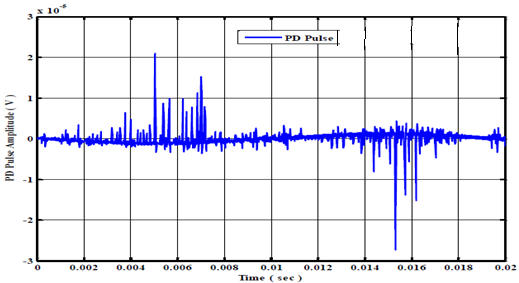
\includegraphics[width=\textwidth]{SineWaveofPartialDischarge}
    \caption{Sine Wave of Partial Discharge }
    \label{fig:Sine Wave of Partial Discharge }
\end{figure}
 
The Partial Discharge pulses are located with reference to the phase angle in positive and negative half cycle with respect to the phase angle.

The partial discharges due to the breakdown of insulation can be distinguished with the partial discharge with different types of discharges. The partial discharge pulses in the different quadrant can lead to a reoccurrence of discharges. With the voltage of 145 kV and different void sizes, the partial discharges pulse are shown in waveforms \cite{Dielectricwithstands}.

Results from the Simulink model has given various Partial discharge pulse, and it is observed that the density of PD is more at the center of positive and negative half cycle.Because of high insulation strength in high voltage Current Transformers, the breakdown in void will cause only when electric stress in the void excess strength of complete insulation. Therefore, PDs mostly appear at the center of half cycle of the sine waveform. 

\begin{figure}[h!]
    \centering
    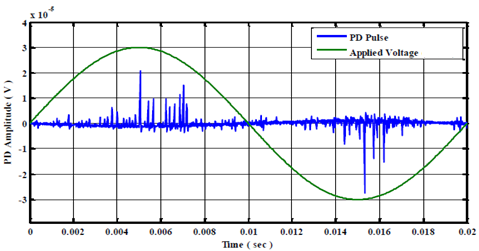
\includegraphics[width=\textwidth]{PartialDischargesinSinusoidalWaveform}
    \caption{Partial Discharges in Sinusoidal Waveform}
    \label{fig:Partial Discharges in Sinusoidal Waveform}
\end{figure}

From the partial discharge pulse for various void dimensions analysis has been done for the magnitude, density of pulse when 145 kV applied for different void sizes\setlength{\parskip}{0em}.

\clearpage
\subsubsection{Simulation waveforms of high voltage current transformers for different void dimensions during steady state conditions}

\begin{figure}[h!]
    \centering
    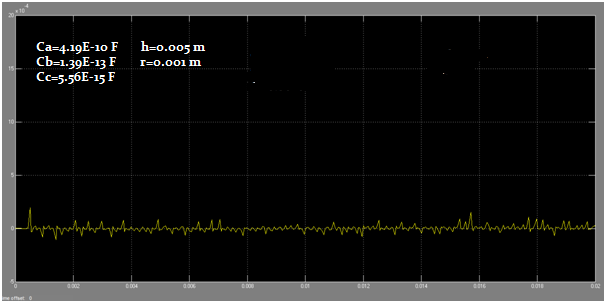
\includegraphics[width=\textwidth]{WaveformsforSteadyState1}\\
    \vspace{1cm}
    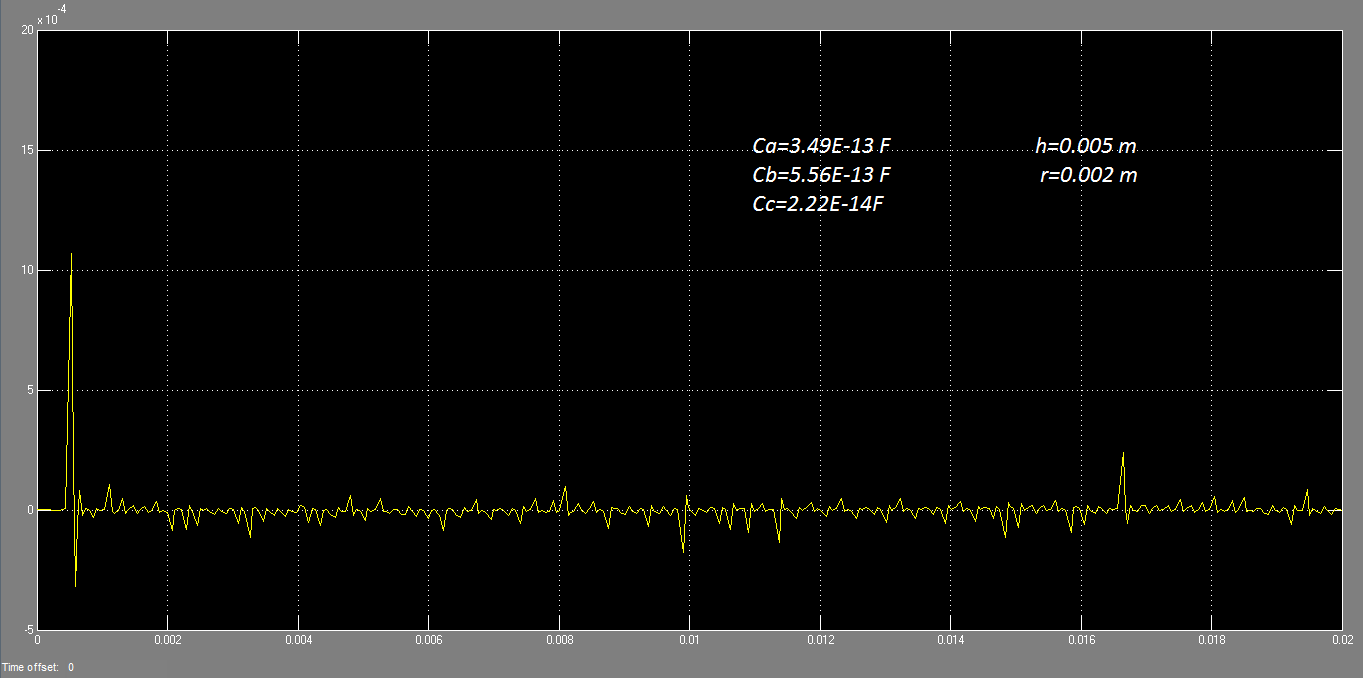
\includegraphics[width=\textwidth]{WaveformsforSteadyState2}
    \caption{Waveforms for Steady State}
    \label{fig:Waveforms for Steady State}
\end{figure}

The amplitude of the Pulse at the initial stage of the Positive waveform has increased as the dimensions of void increases.

\begin{center}
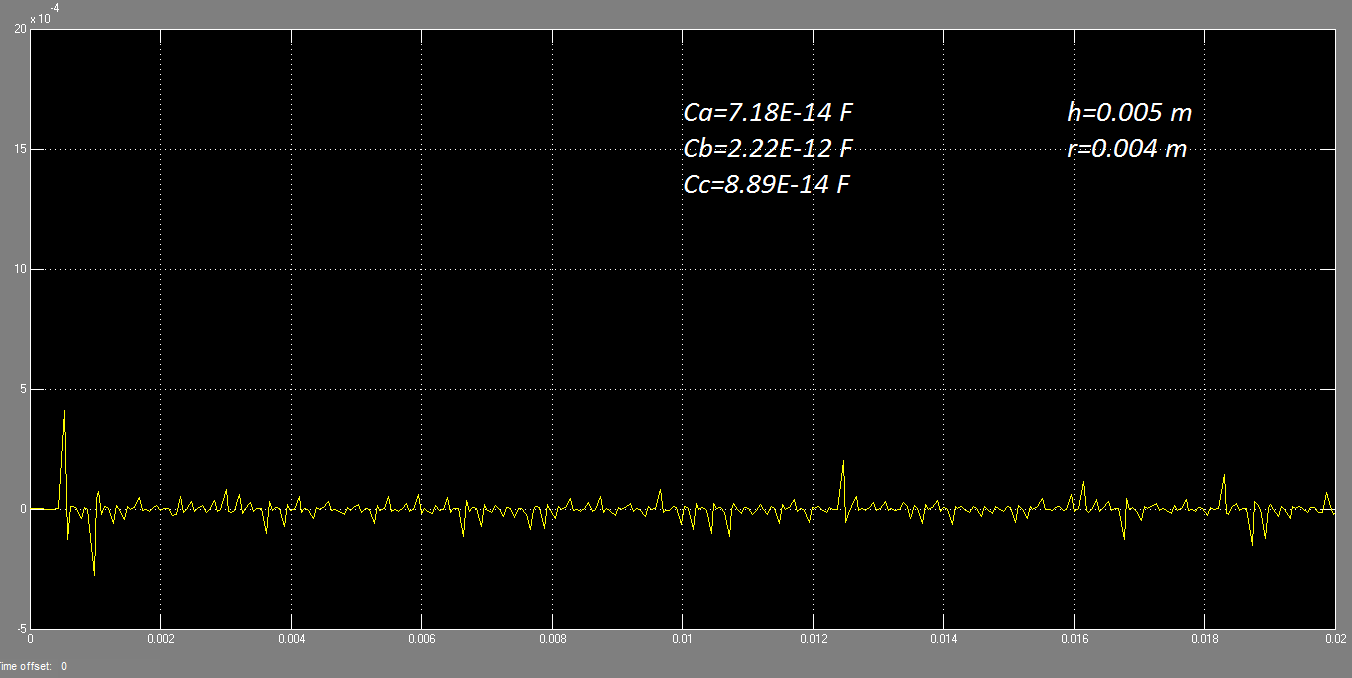
\includegraphics[width=\textwidth]{Wave3}
\vfill
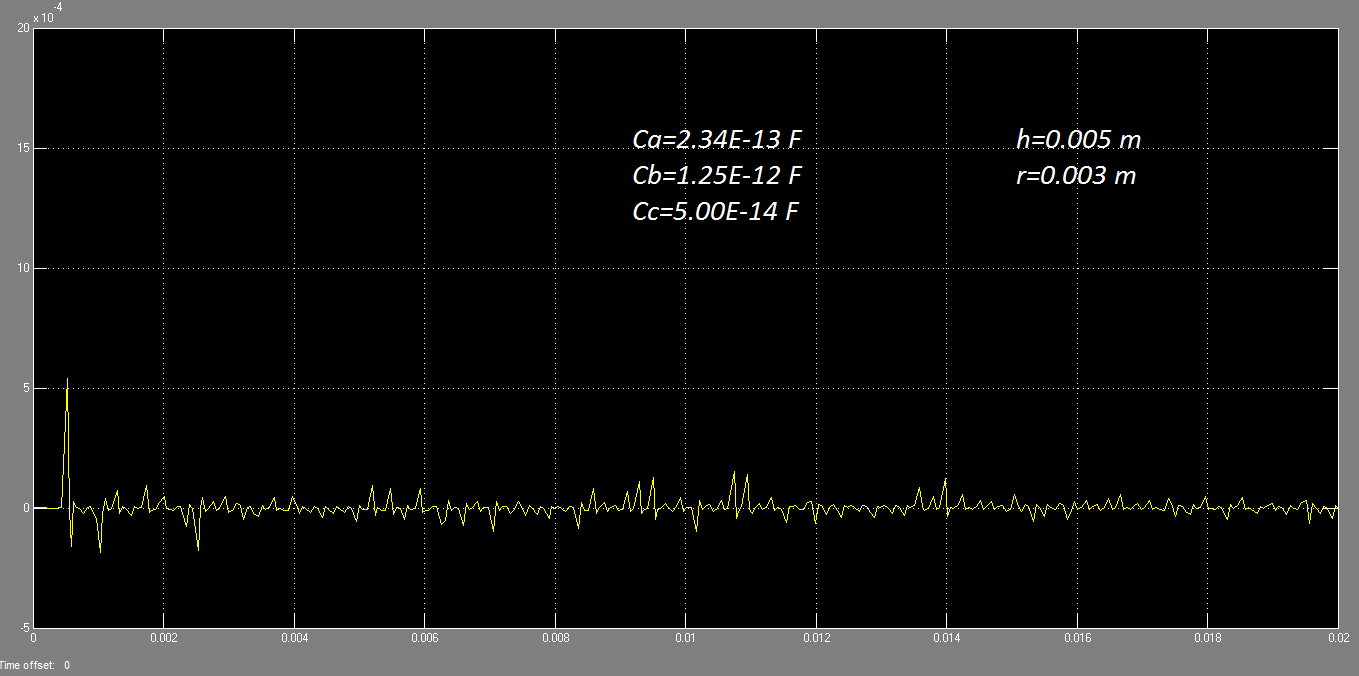
\includegraphics[width=\textwidth]{Wave4}
\vfill
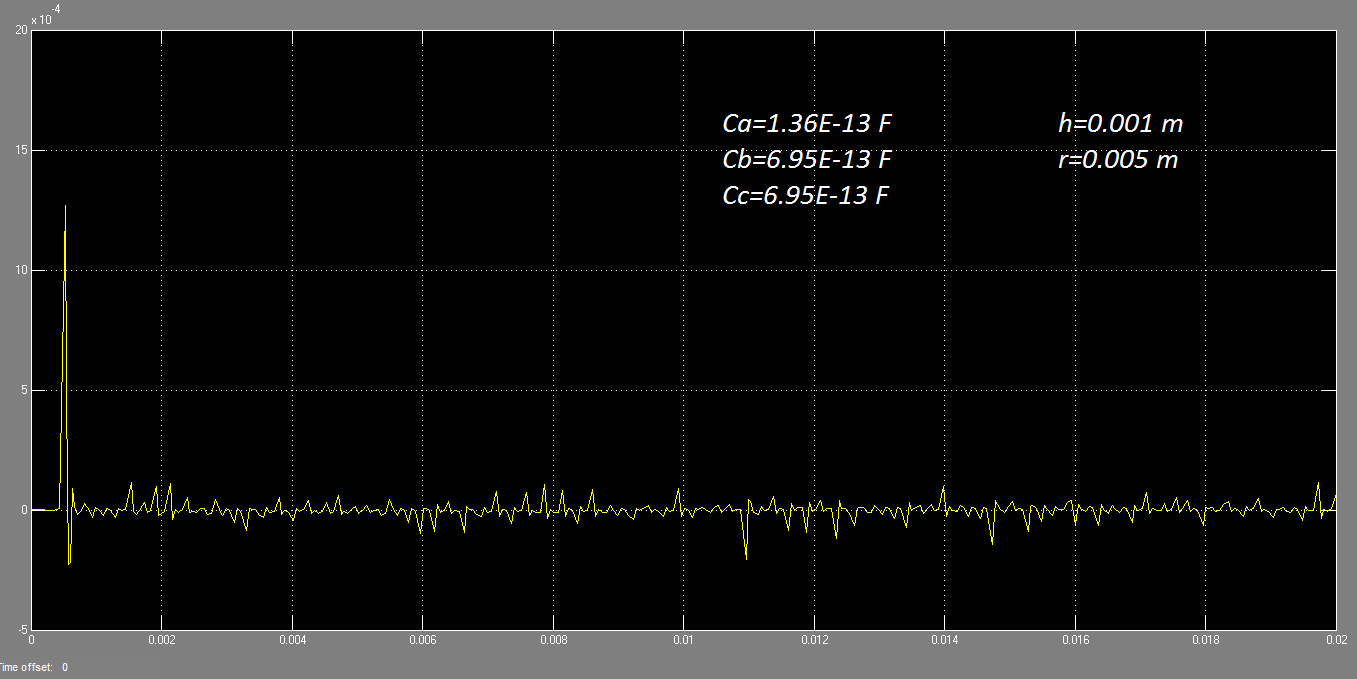
\includegraphics[width=\textwidth]{Wave5}
\end{center}
A number of PD Pulse Count is more in Negative Pulse.
The PD Level Waveform increases with increase in void dimensions.
\pagebreak

\begin{center}
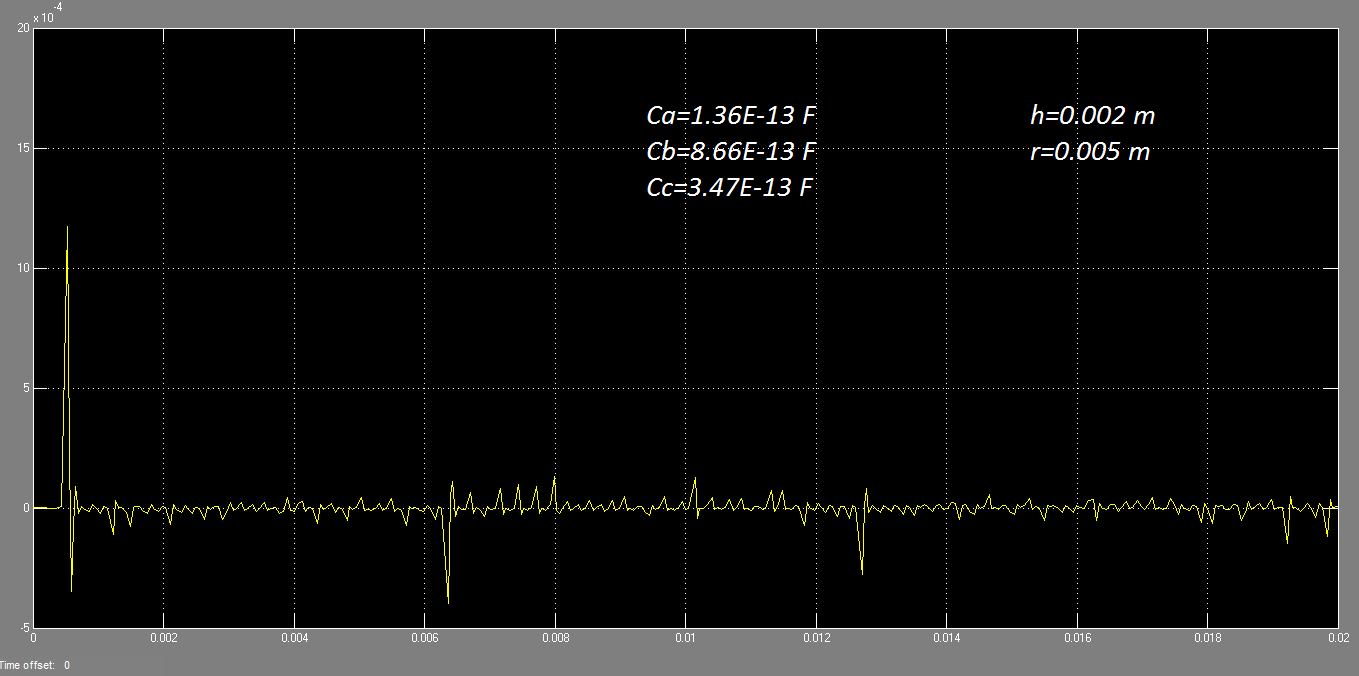
\includegraphics[width=\textwidth]{Wave6}
\vfill
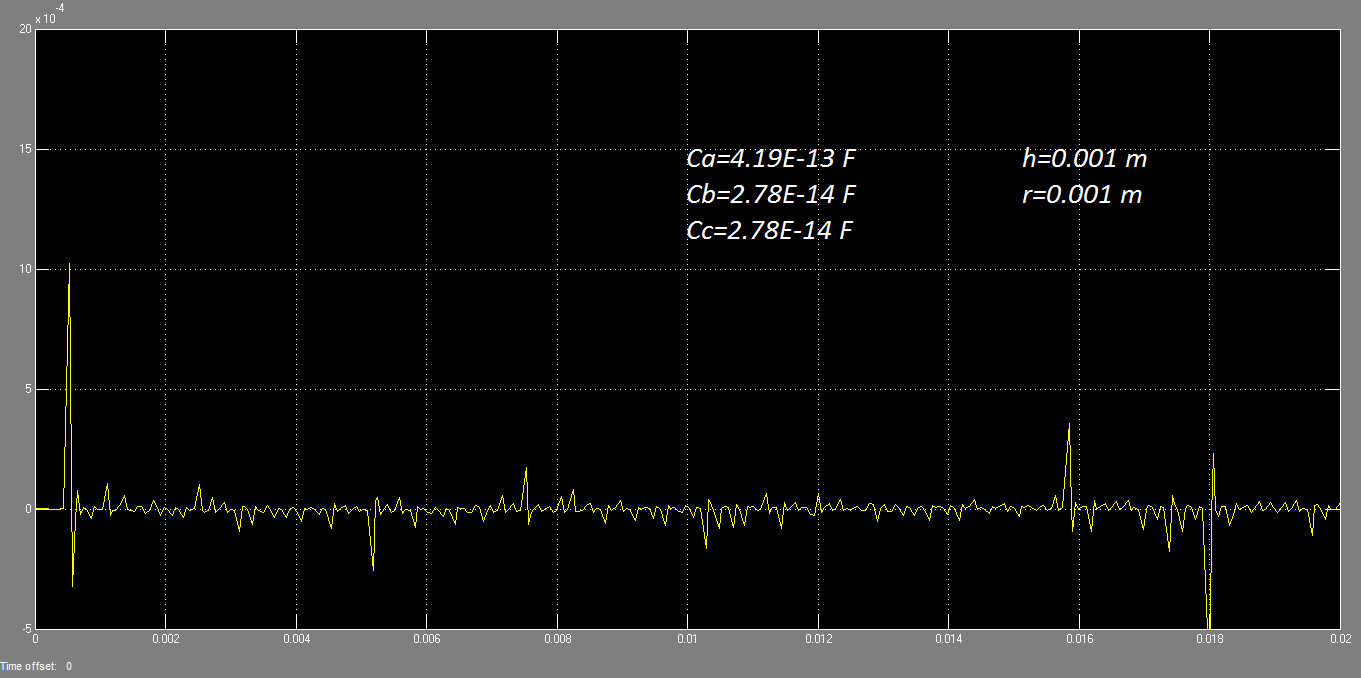
\includegraphics[width=\textwidth]{Wave7}
\vfill
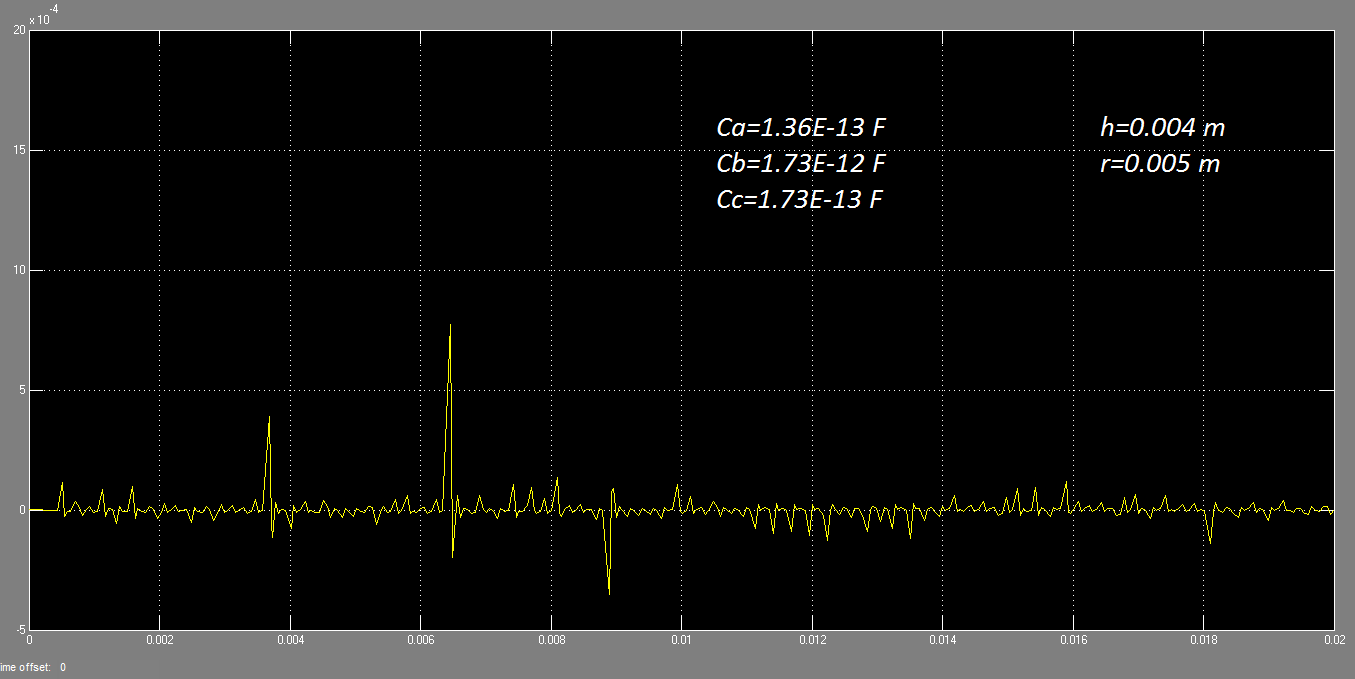
\includegraphics[width=\textwidth]{Wave8}
\end{center}

\pagebreak
\begin{center}
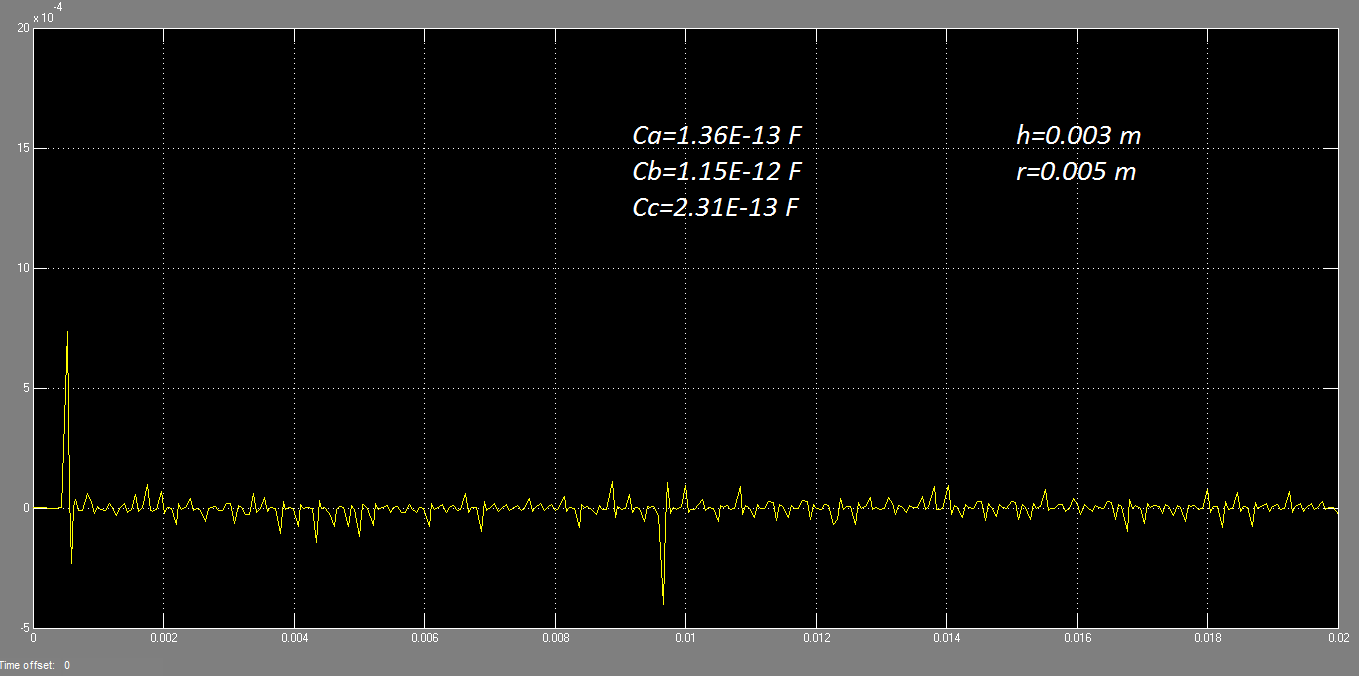
\includegraphics[width=\textwidth]{Wave9}
\vfill
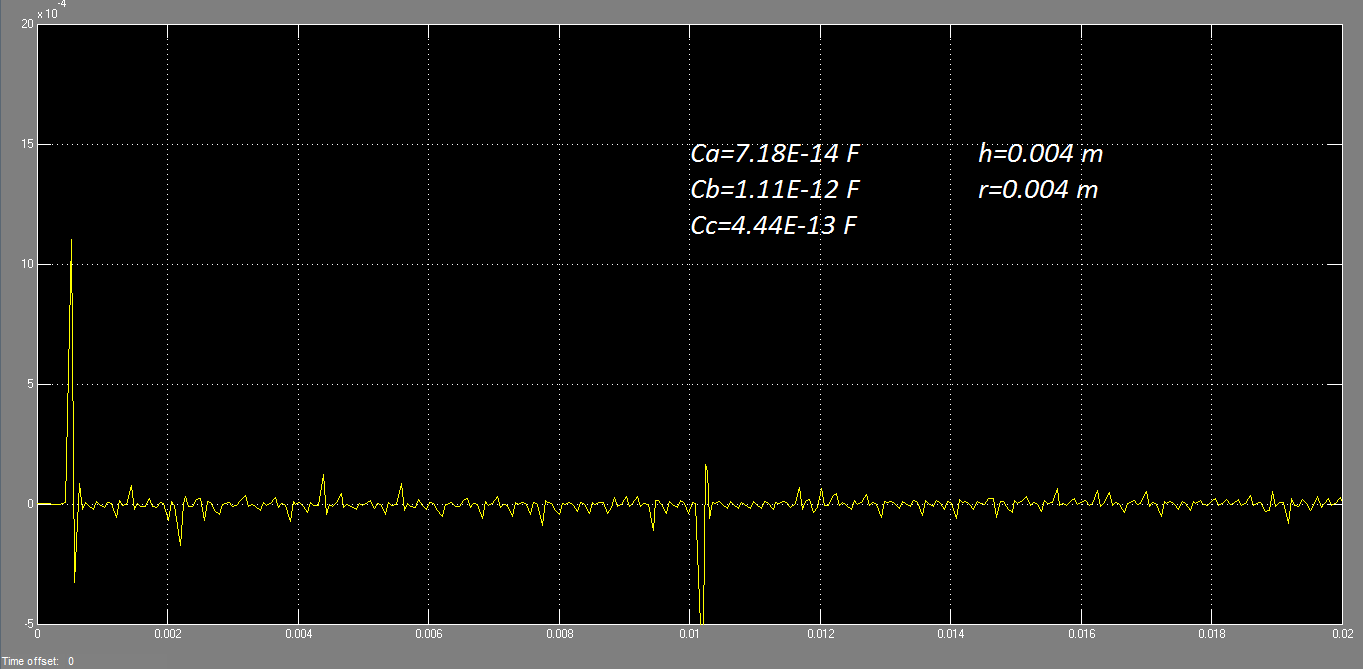
\includegraphics[width=\textwidth]{Wave91}
\vfill
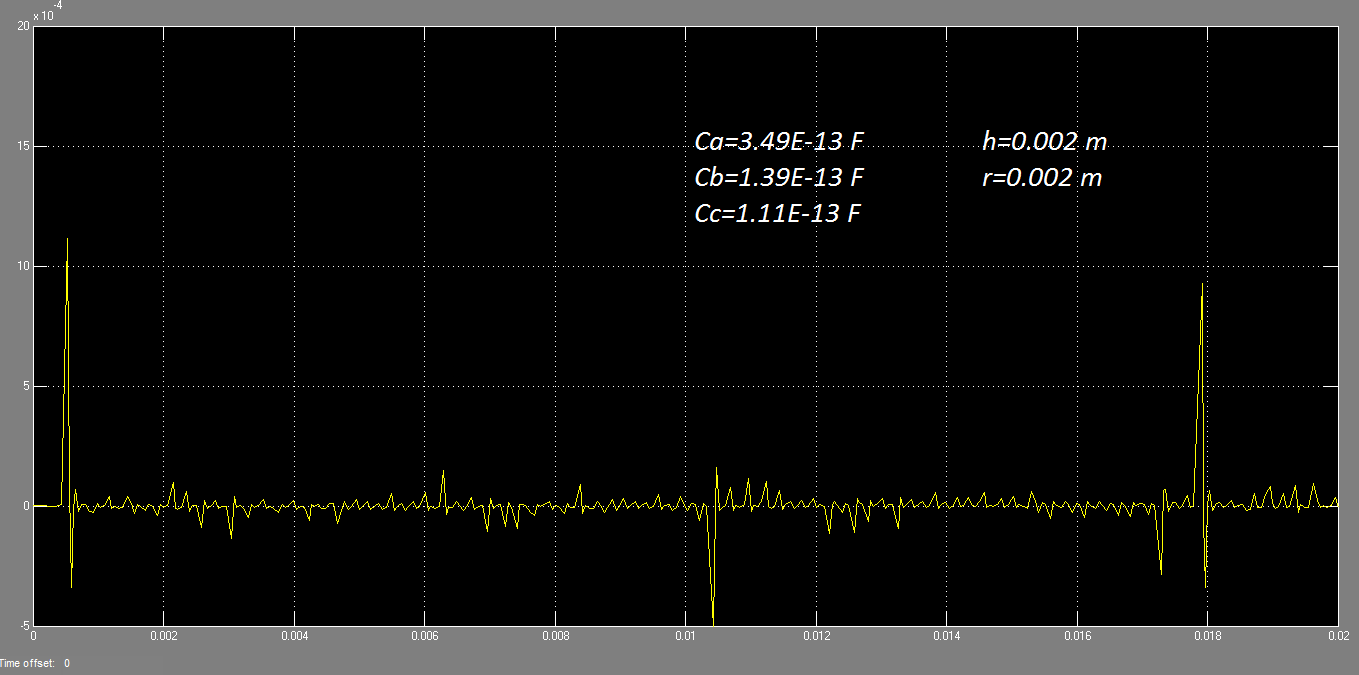
\includegraphics[width=\textwidth]{Wave92}
\end{center}

\pagebreak
\begin{center}
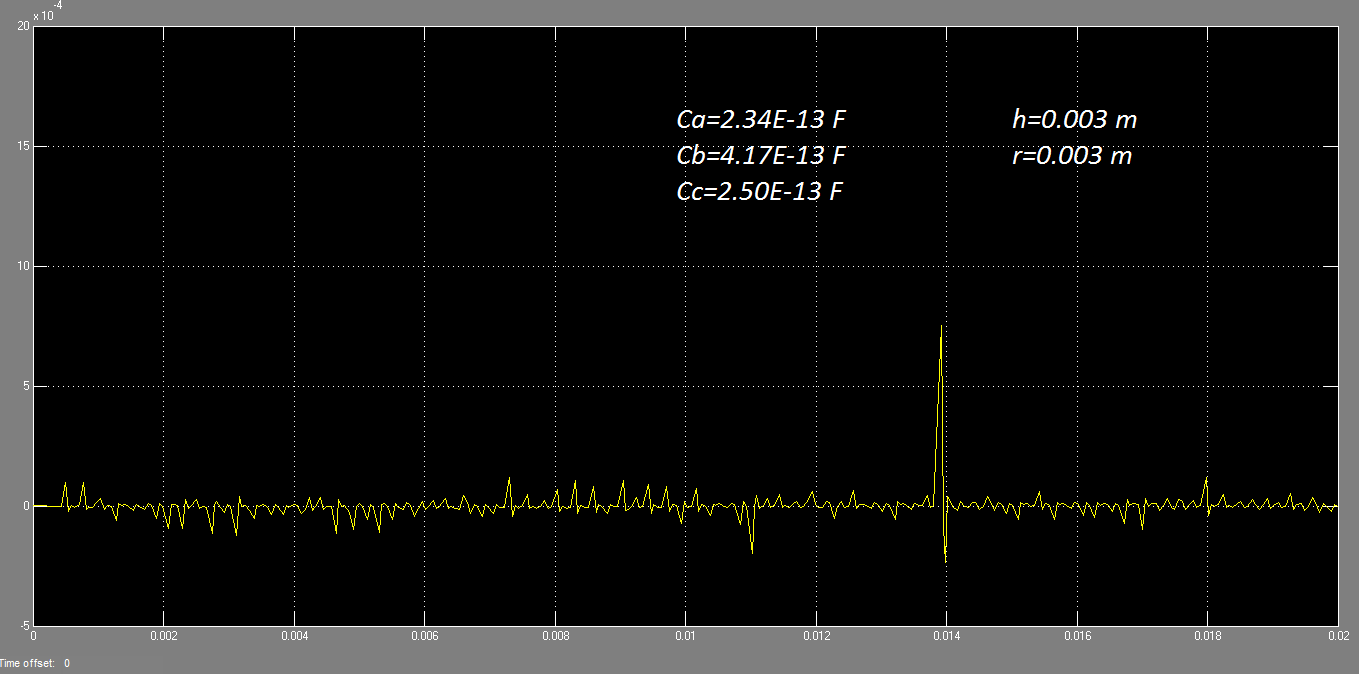
\includegraphics[width=\textwidth]{Wave93}
\vfill
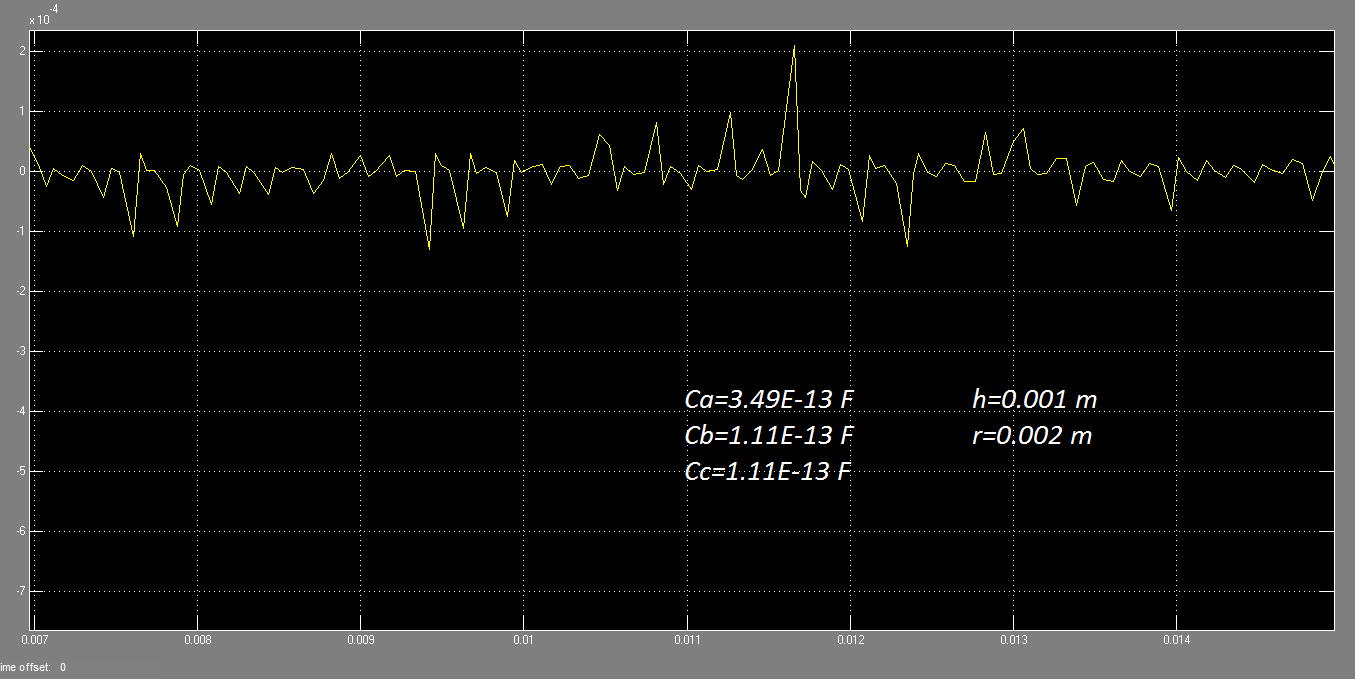
\includegraphics[width=\textwidth]{Wave94}
\vfill
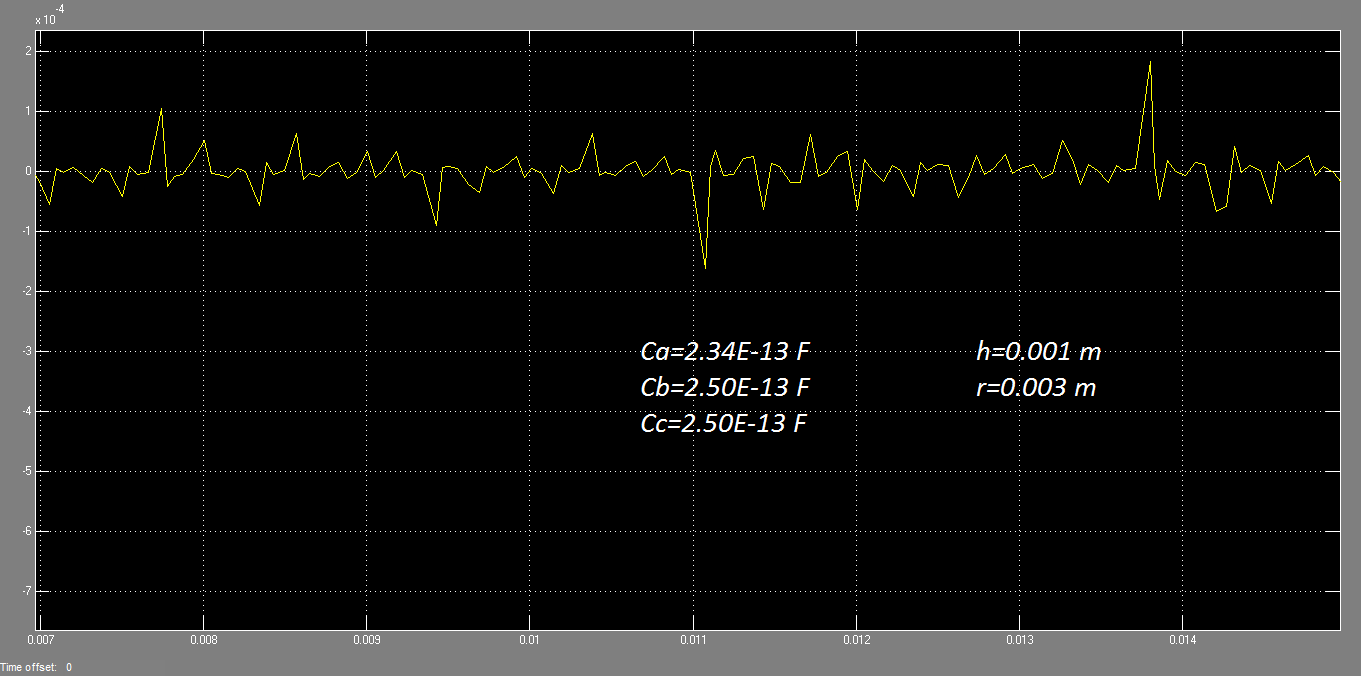
\includegraphics[width=\textwidth]{Wave95}
\end{center}

The amplitude of the PD Pulse increases with increase in the waveform.

\pagebreak
\begin{center}
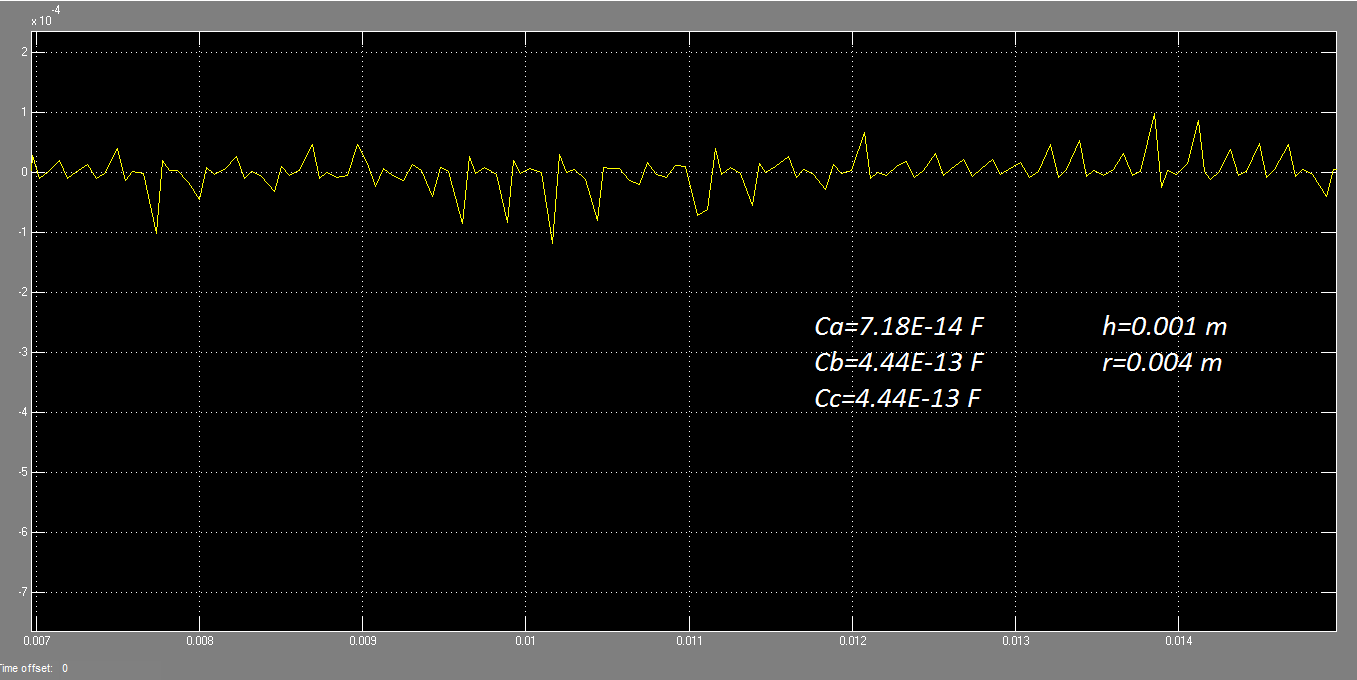
\includegraphics[width=\textwidth]{Wave96}
\vfill
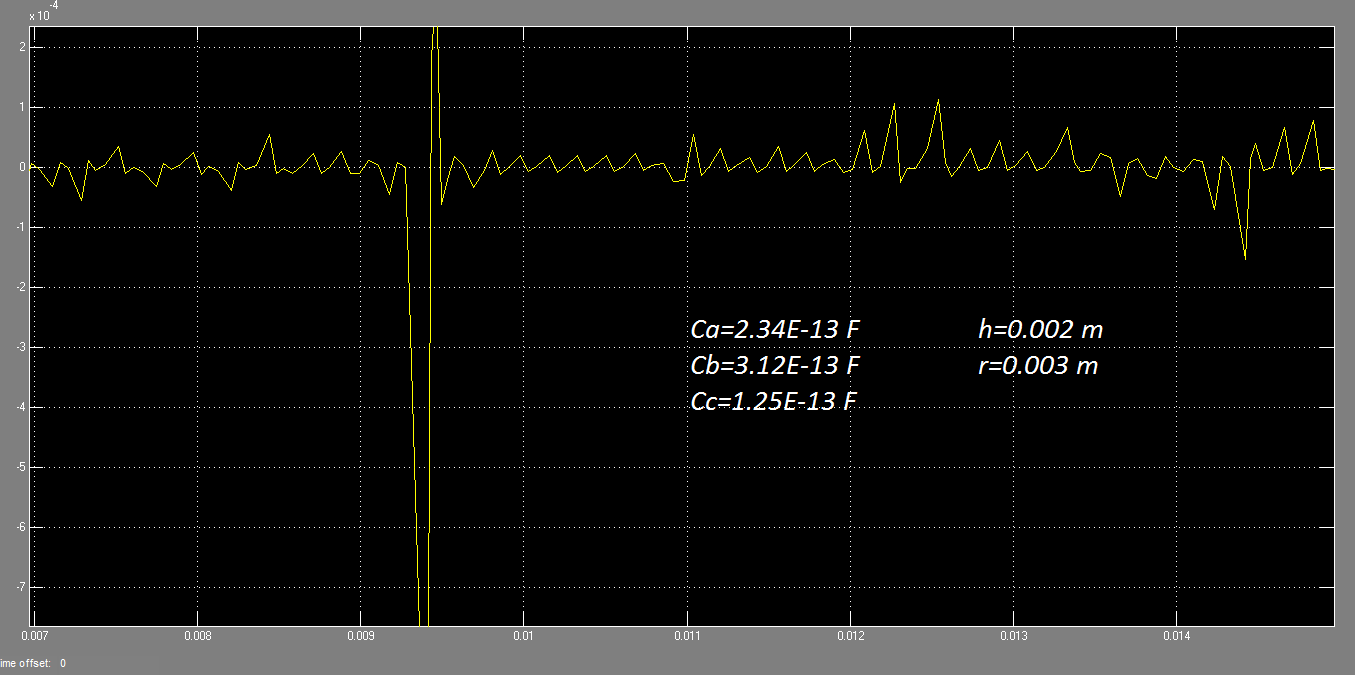
\includegraphics[width=\textwidth]{Wave97}\\
Partial Discharge waveform is more in number as the dimensions of the void are more.
\vfill
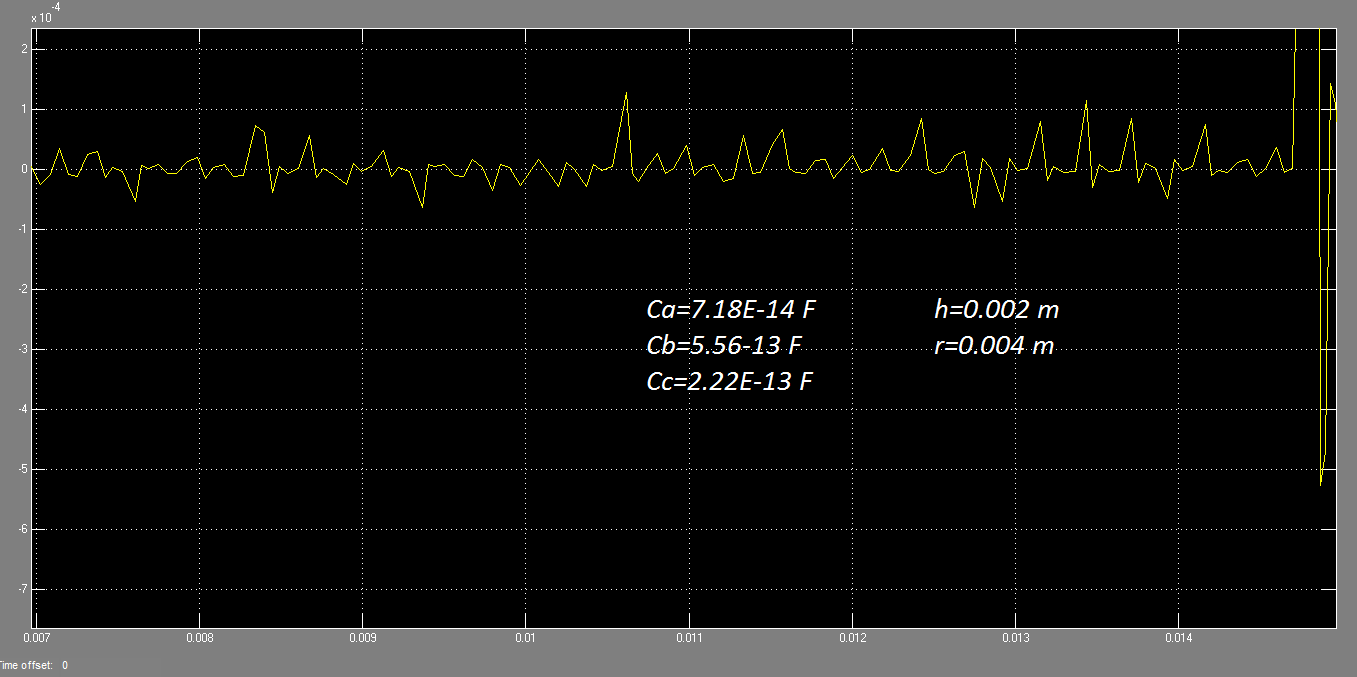
\includegraphics[width=\textwidth]{Wave98}
\end{center}

\pagebreak
\begin{center}
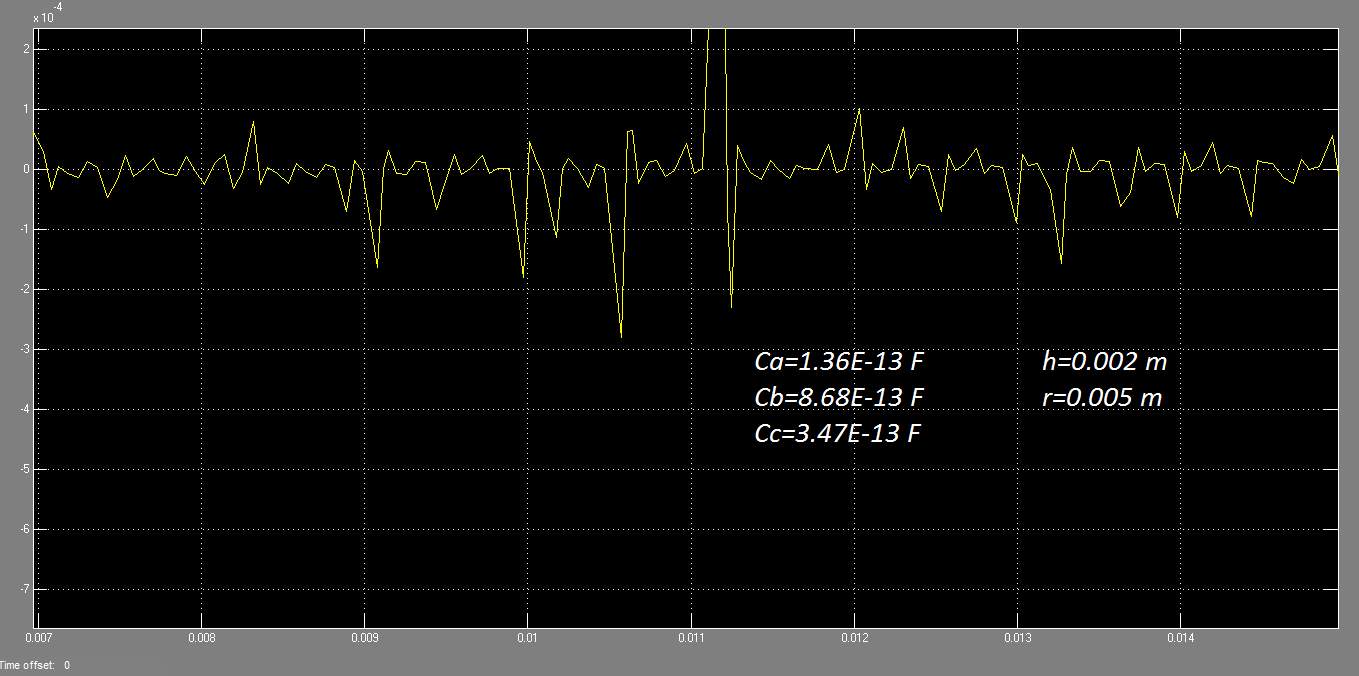
\includegraphics[width=\textwidth]{Wave99}
\vfill
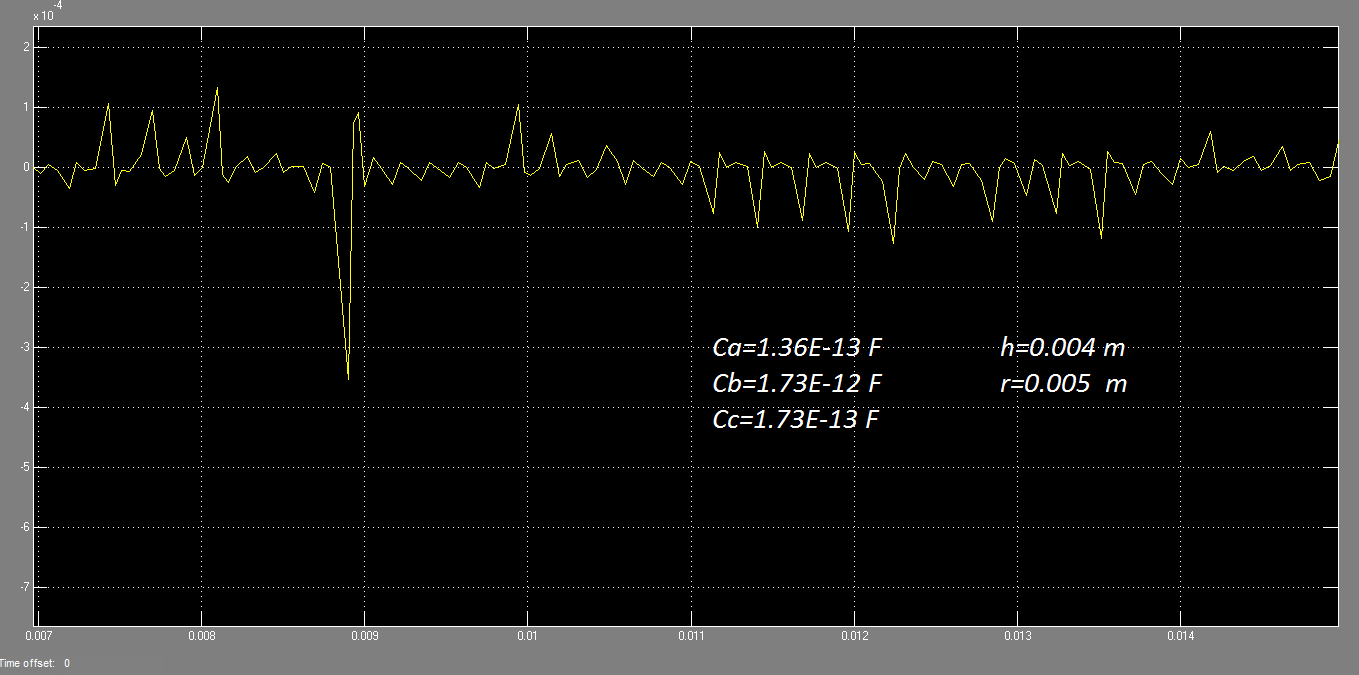
\includegraphics[width=\textwidth]{Wave991}
\vfill
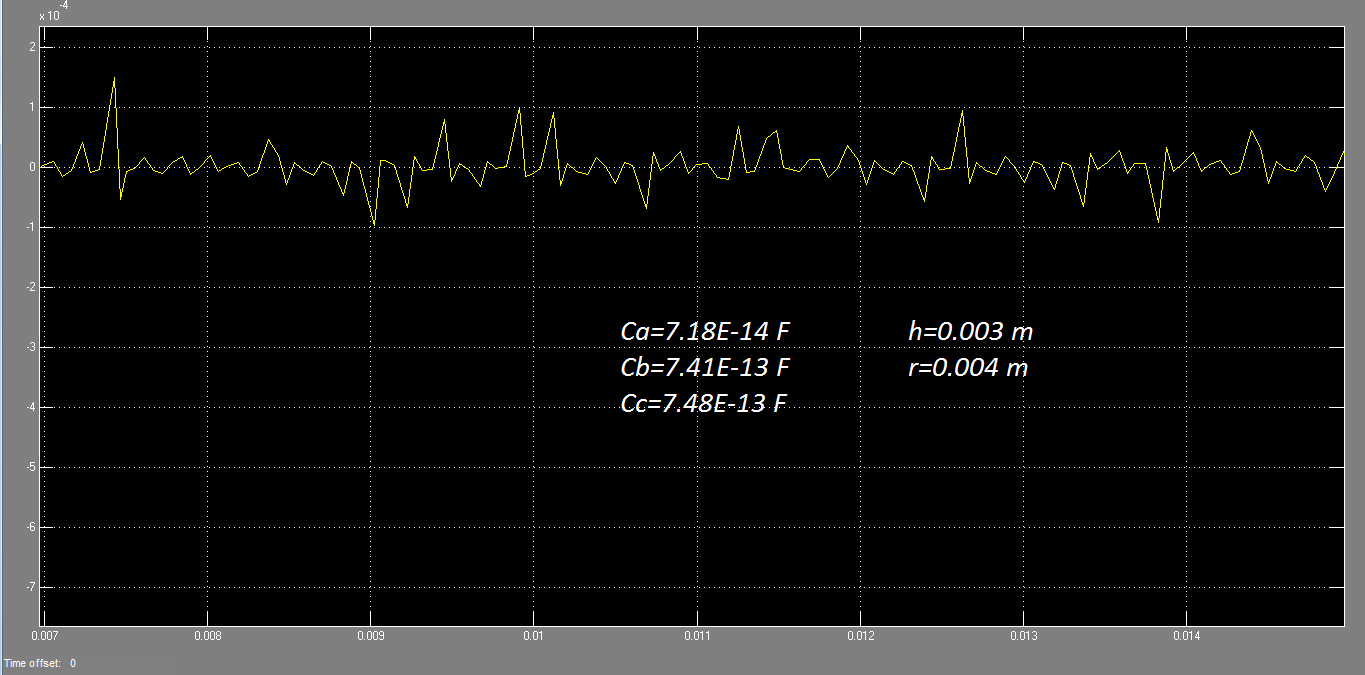
\includegraphics[width=\textwidth]{Wave992}
\end{center}

\pagebreak
\begin{center}
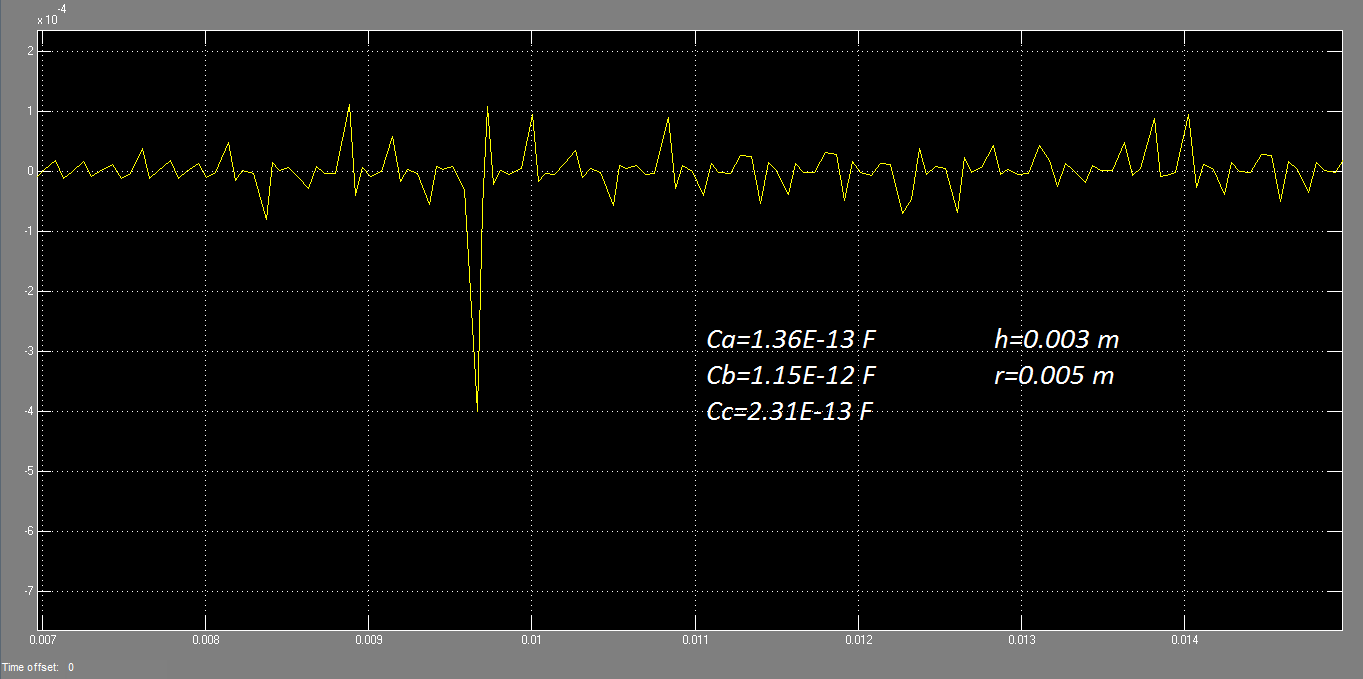
\includegraphics[width=\textwidth]{Wave993}
\vfill
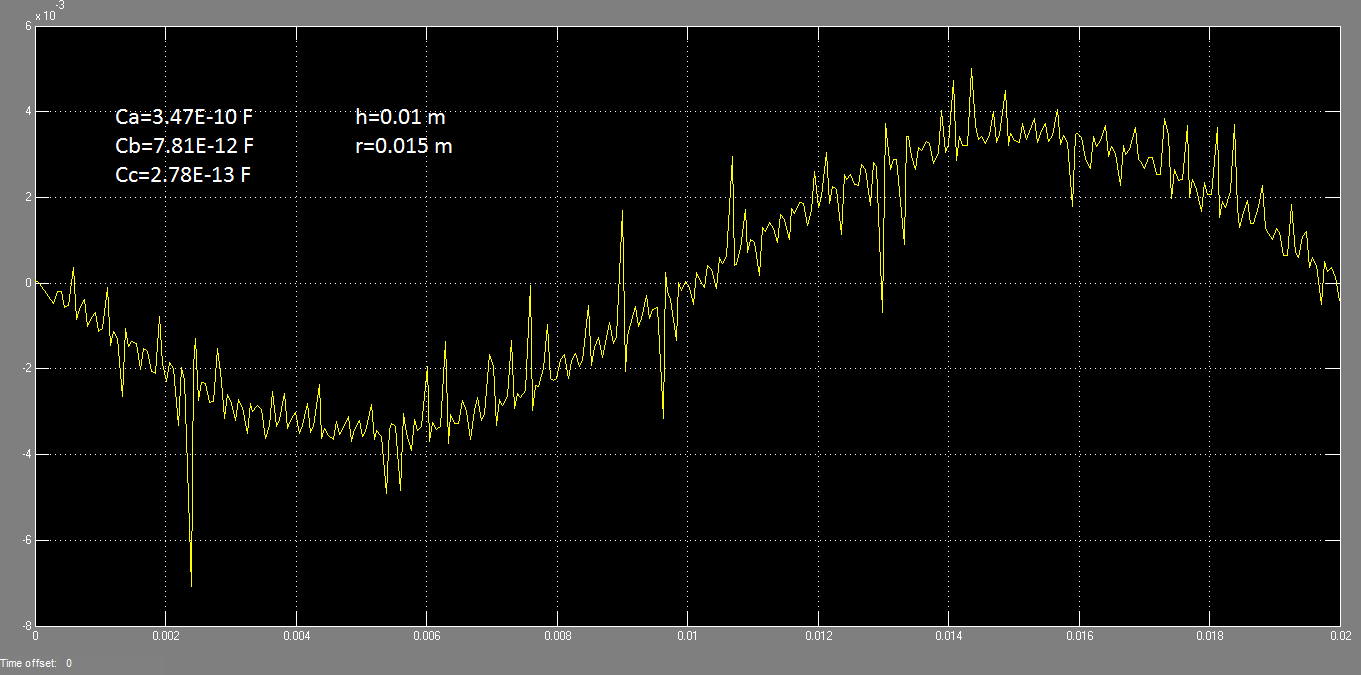
\includegraphics[width=\textwidth]{Wave994}
\vfill
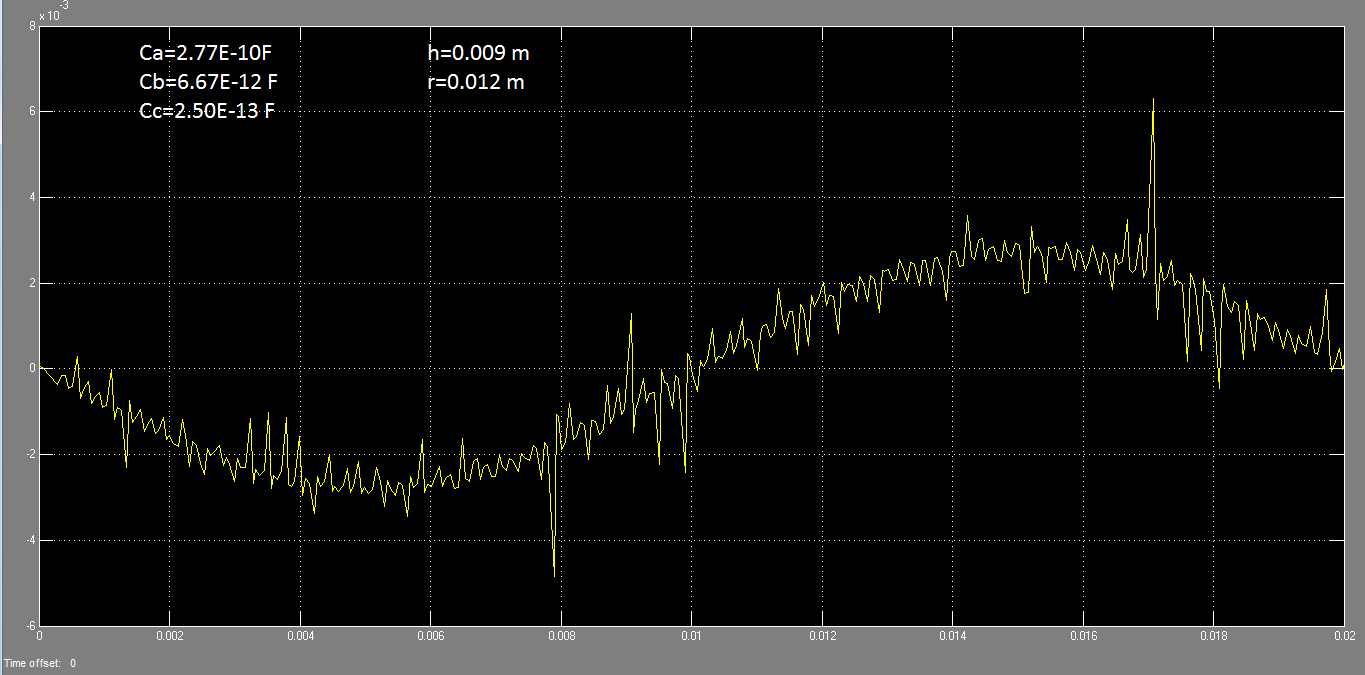
\includegraphics[width=\textwidth]{Wave995}
\end{center}

\pagebreak
\begin{center}
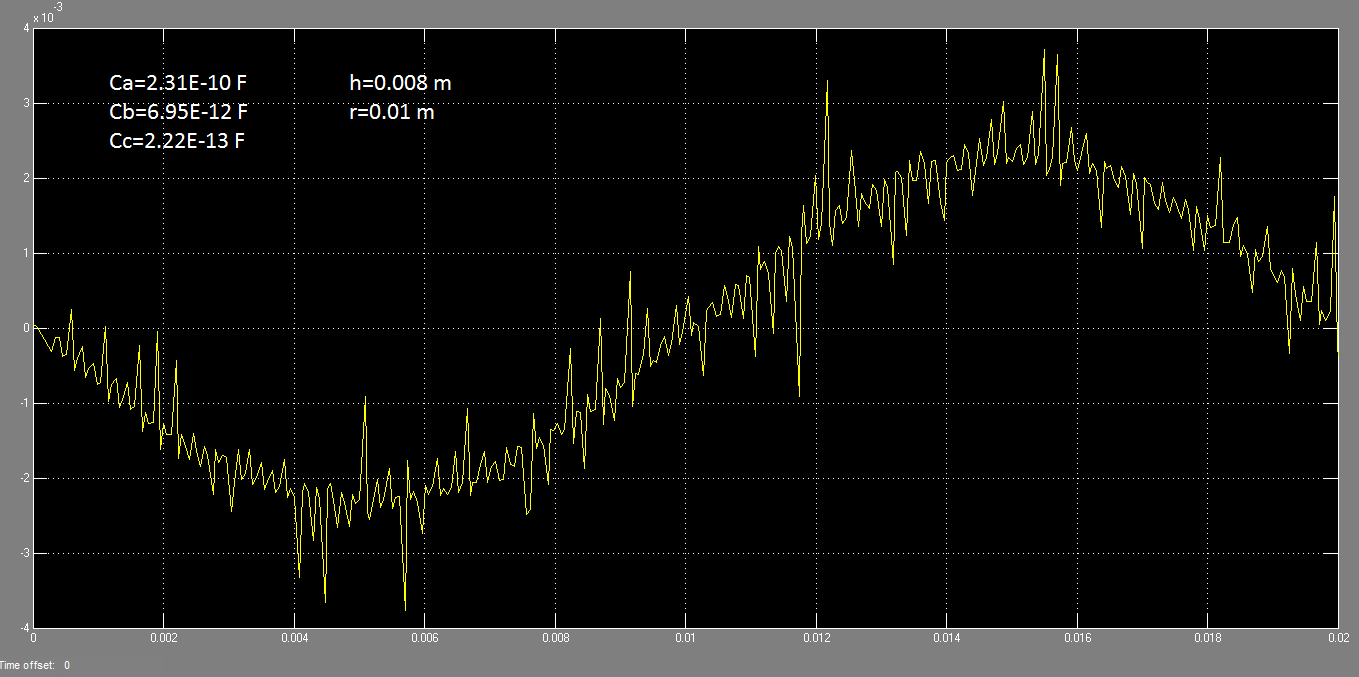
\includegraphics[width=\textwidth]{Wave996}
\vfill
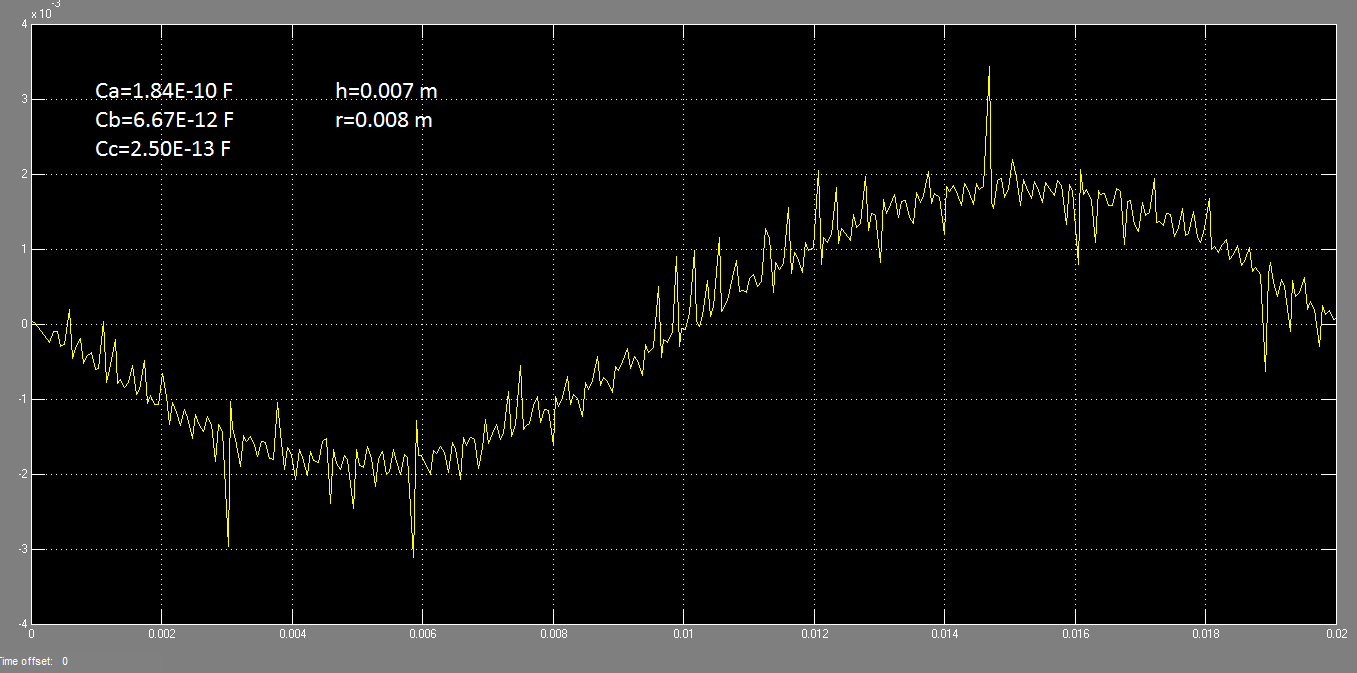
\includegraphics[width=\textwidth]{Wave997}
\vfill
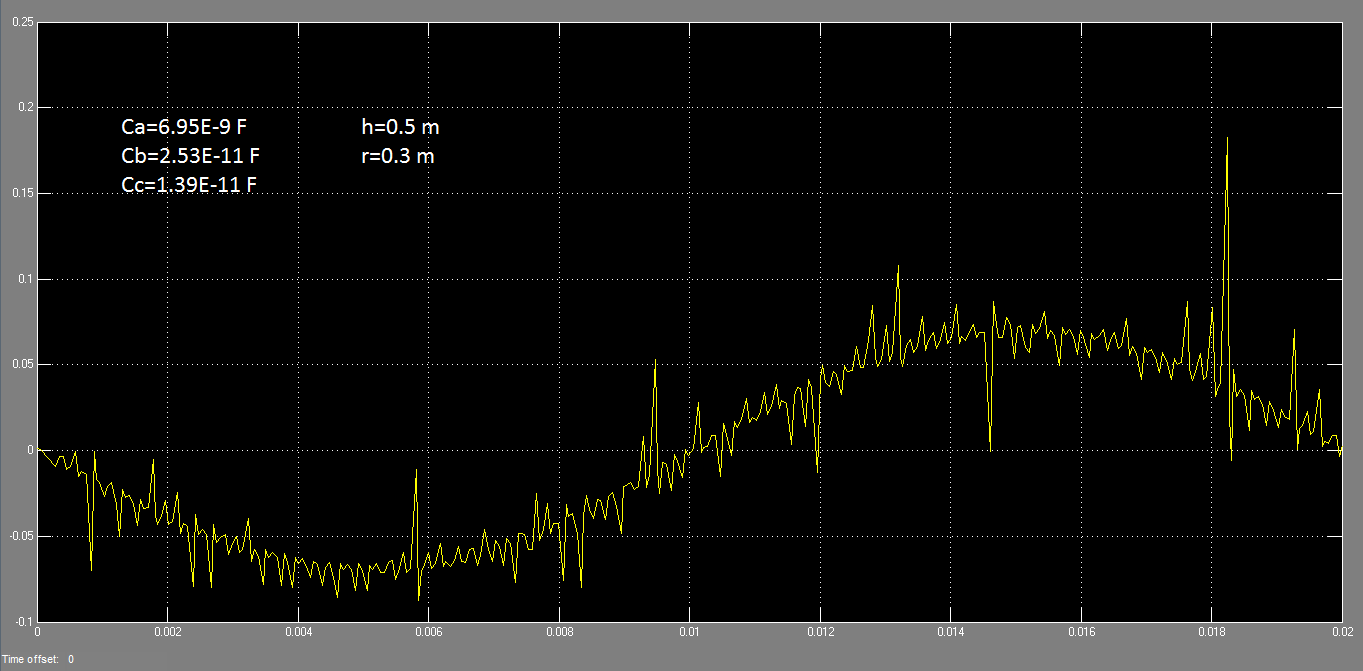
\includegraphics[width=\textwidth]{Wave998}
\end{center}

\pagebreak
\begin{center}
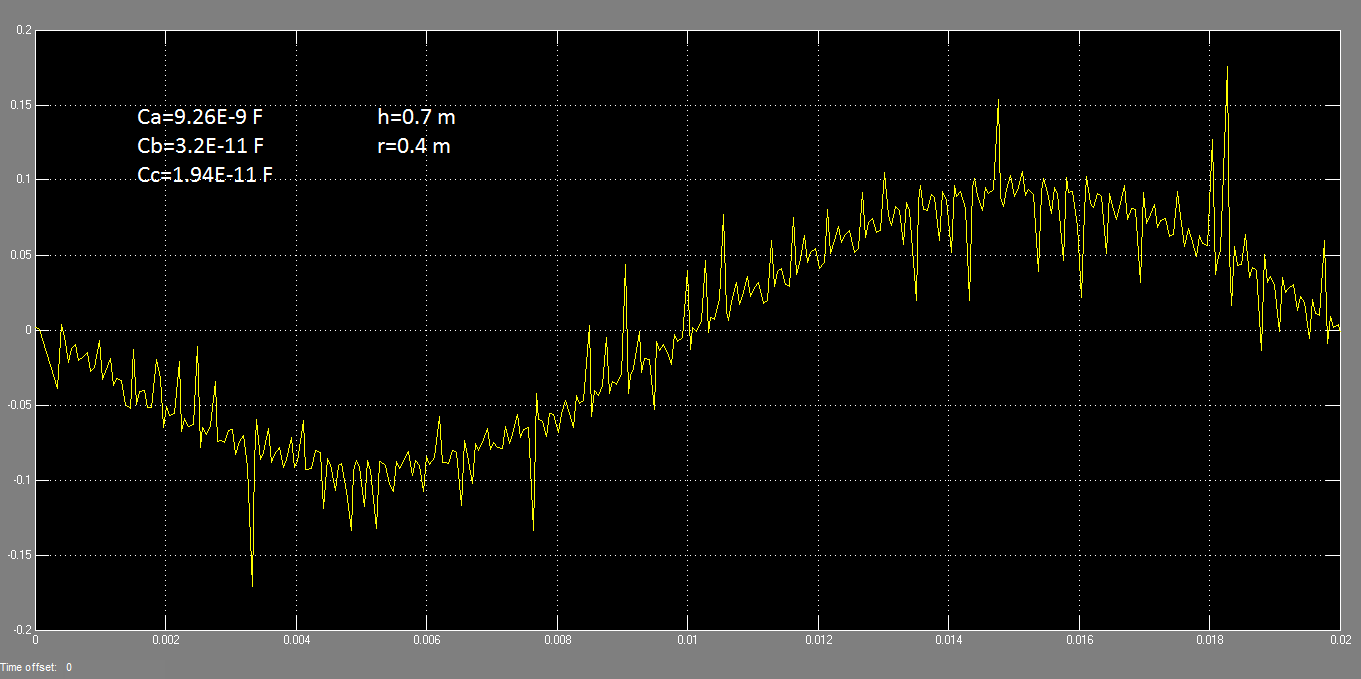
\includegraphics[width=\textwidth]{Wave999}\\
Amplitude and frequency of PD waveform increase for higher void sizes. 
The Density of PD waveform, Pulses are more.
\vfill
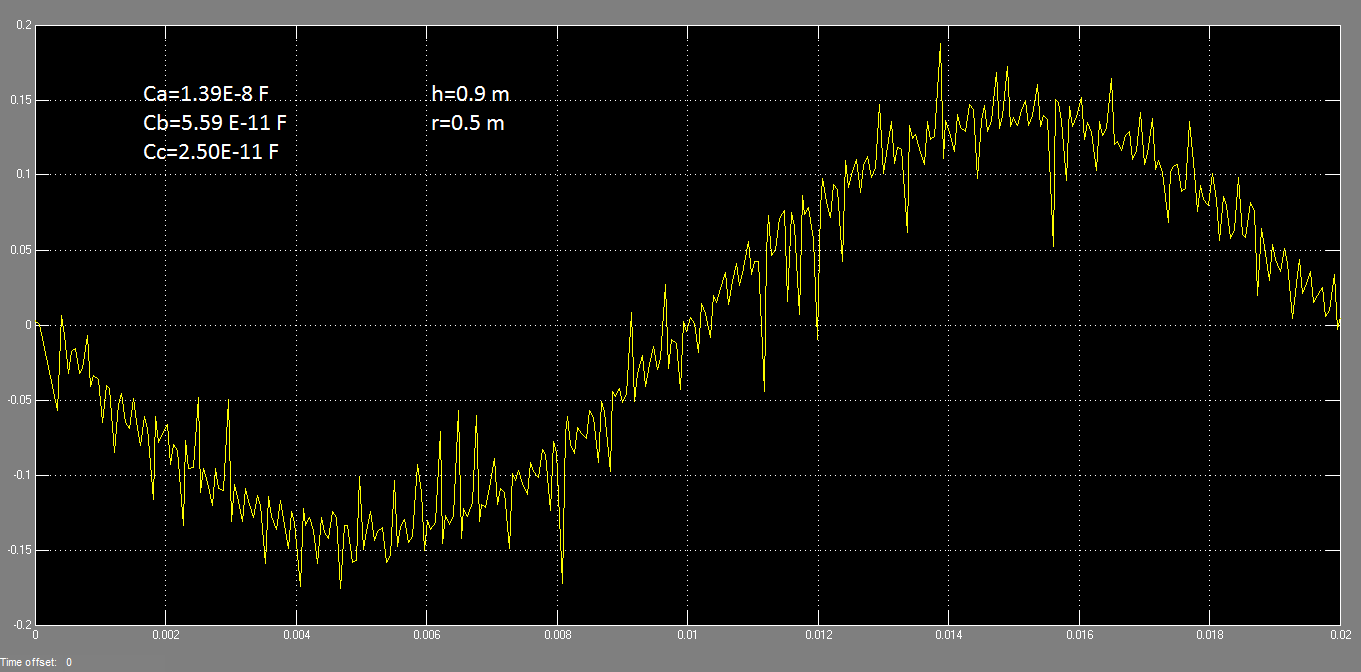
\includegraphics[width=\textwidth]{Wave9991}
\vfill
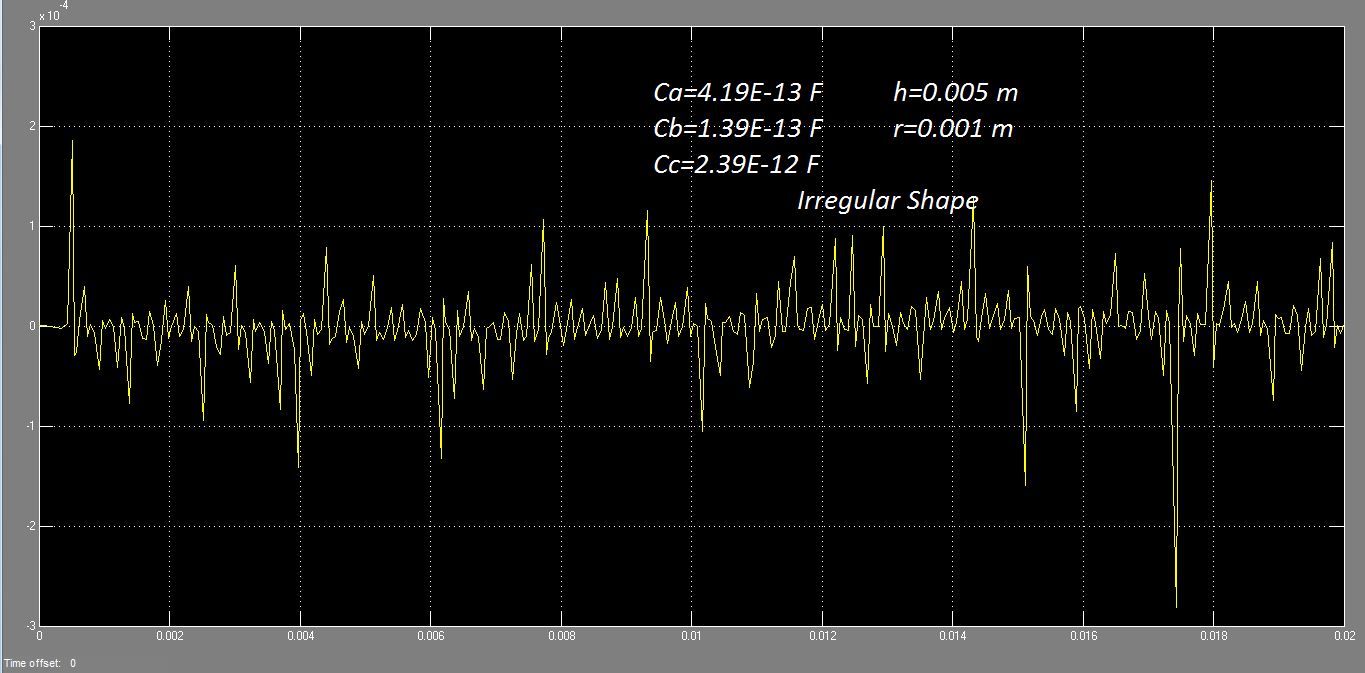
\includegraphics[width=\textwidth]{Wave9992}
\end{center}

\pagebreak
\begin{center}
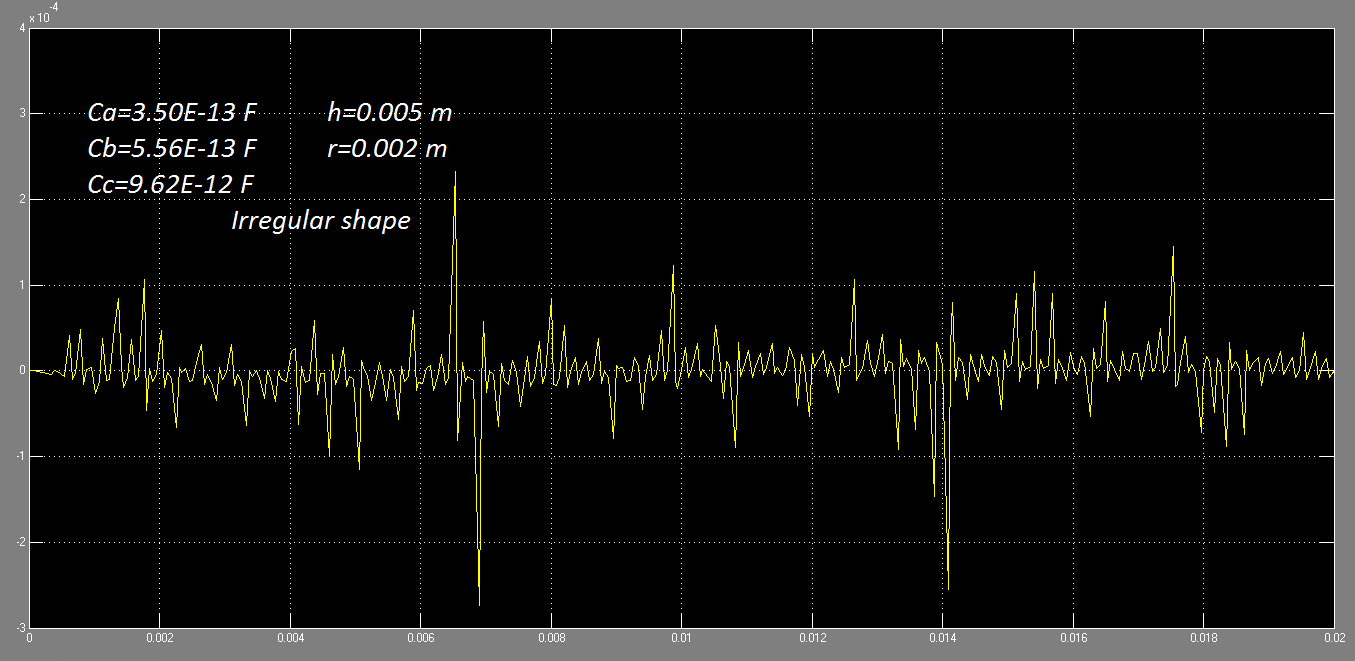
\includegraphics[width=\textwidth]{Wave9993}
\vfill
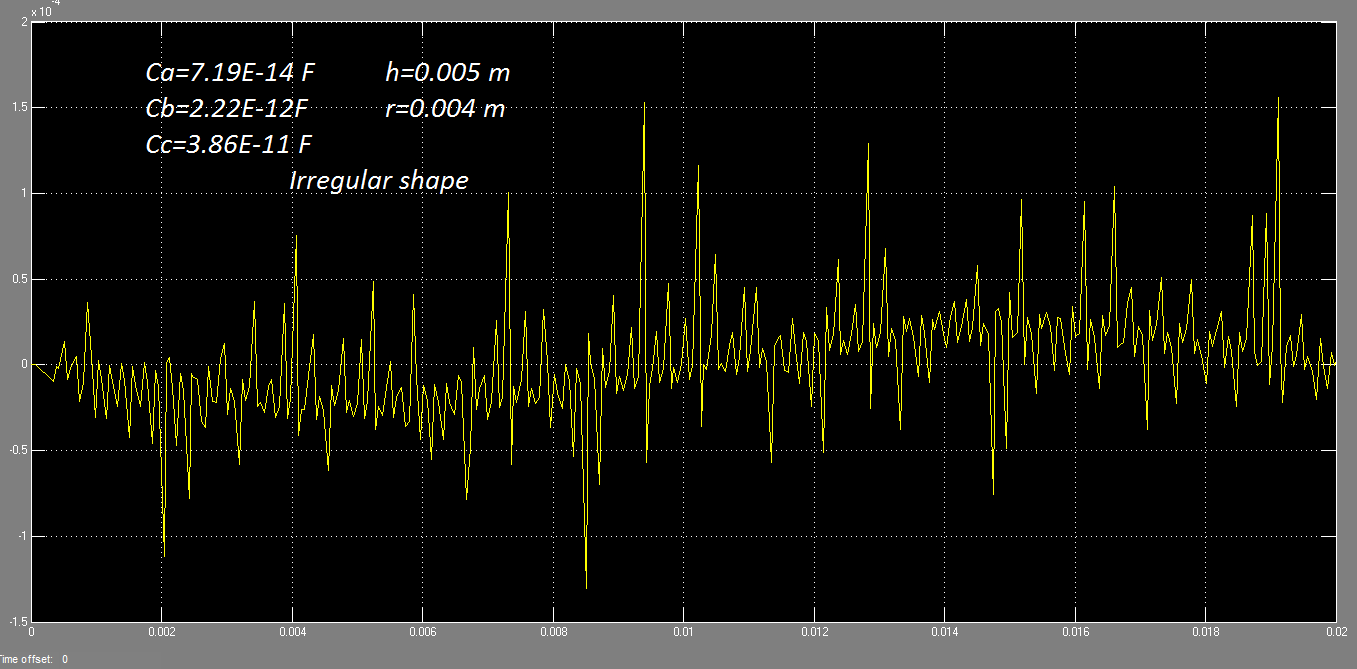
\includegraphics[width=\textwidth]{Wave9995}
\vfill
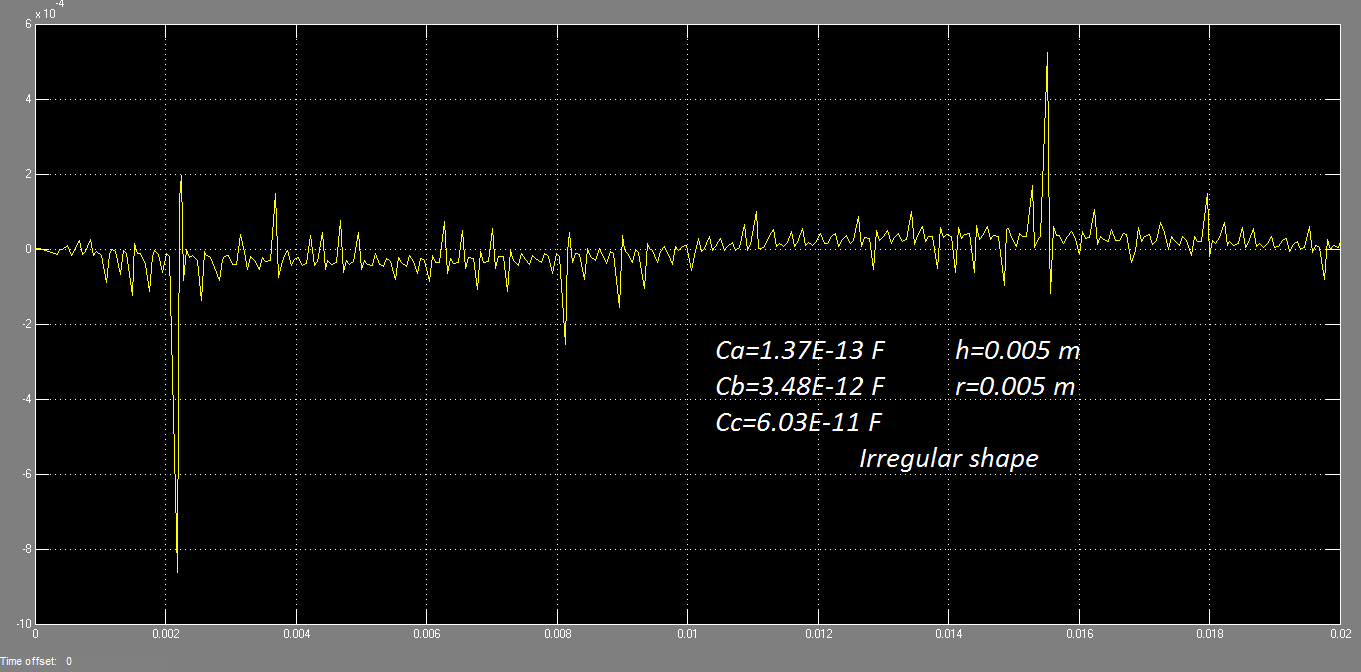
\includegraphics[width=\textwidth]{Wave9996}
\end{center}

\subsection[Analysis of simulation model for high voltage current transformers in short circuit and transient condition]{Analysis of simulation model for high voltage\\current transformers in short circuit and\\transient condition}

The performance of partial discharge was studied in short circuit and transient condition with Simulink model. The voltage of 145 kV was applied, and different void was provided in Simulink. The Capacitance values calculated as per the Table \ref{table:Values of Capacitance for Different Void Sizes} for $C_a$, $C_b$, $C_c$. System was run for the partial discharge pulses\setlength{\parskip}{1em}.

Enclosed ~all ~samples ~of ~partial ~discharge ~pulses ~waveform ~for ~different ~void conditions.

From the waveforms for different voids and calculated capacitance the magnitude of partial discharge changes with height, diameter and volume of the void. The capacitance changes with a change in dimensions of the void.

The capacitance values of different void sizes were calculated and shown in the table \ref{table:Values of Capacitance for Different Void Sizes}. The wave form for different capacitances is enclosed.

Conclusions from Simulation with Short Circuit and Transients Generated on Performance of Current Transformer

For various dimensions of voids and calculated capacitance $C_a$, $C_b$, $C_c$ Simulink model was run for short circuit and transient conditions on the system. The transients are a sudden short circuit in the line circuit. In this Simulink model, the magnetizing inductance and magnetizing current have been taken into account.

The Partial discharge activity inside the insulation of current transformer in a MATLAB Simulink model has taken for analysis and evaluation.

\begin{enumerate}
\item The Partial discharge activity inside the high voltage current transformers solid or oil insulation depends on the size of the void presence inside the oil and paper. The values of partial discharge increase with the voltage given to current transformer.

\item The PD waveform wave generated for different void were studied for magnitude, number, PD distribution and frequency of pulses.

\item In the Simulink model for Short circuit and Transient conditions, various capacitance values are put, and the system was run for the partial discharge waveform.

\item With change in Void parameters and voltage level Partial Discharge pulses varies, the density of PD's also varies

\item In ~high ~voltage ~current ~transformers ~the ~Partial ~Discharge ~can ~lead ~to deterioration of insulating material which can lead to the breakdown of live components in the long term.

\item The partial discharge process will change the properties of oil and other insulating media. With continuous discharge will leads to decomposition and pollution of the insulating oil as a result of which the insulation properties of the oil changes rapidly. 

\item Partial discharge measurement concludes the quality and strength of insulation inside the current transformers.

\item Specific phase related representation and assist and measure the identification of fault type 

\item PD pulse observed for 50 kV, 75 kV, 100 kV and 145 kV applied voltage between the test object has given different PD pulses for same void conditions\setlength{\parskip}{0em}.
\end{enumerate}
\pagebreak 

\subsubsection{Simulation waveforms of high voltage current transformers for different void dimensions during short circuit and transients}

\begin{figure}[h!]
    \centering
    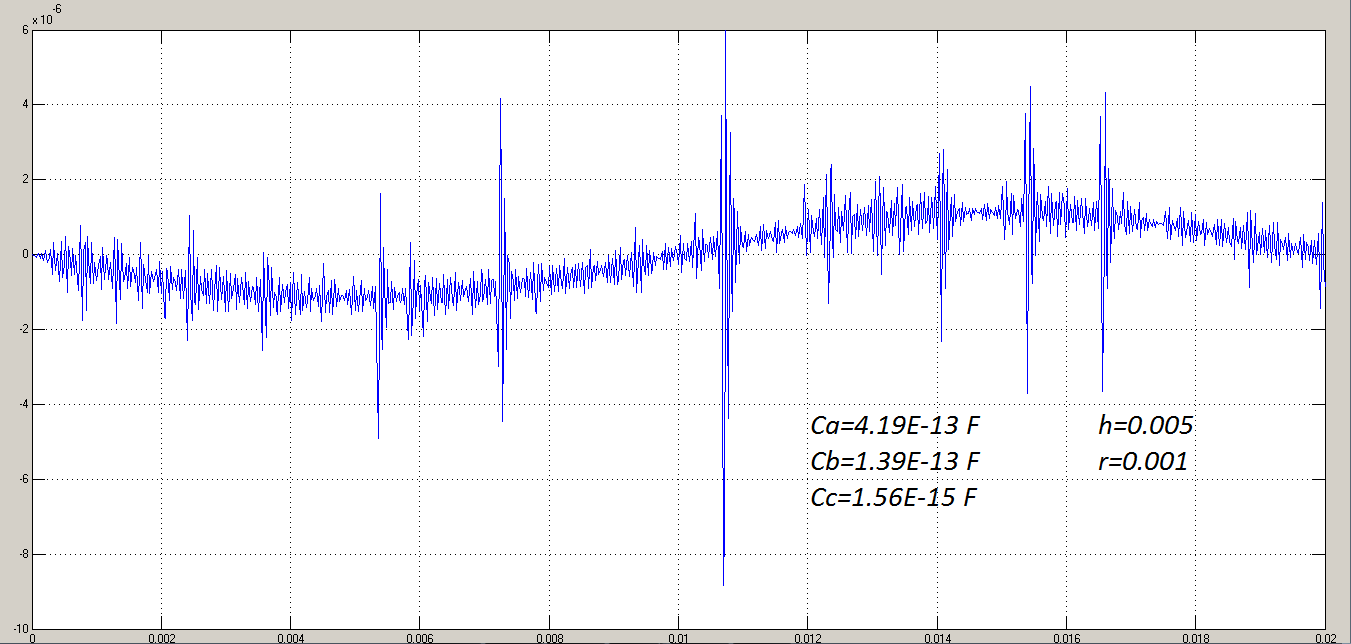
\includegraphics[width=\textwidth]{WaveformsforTransient1}\\
    \vspace{1cm}
    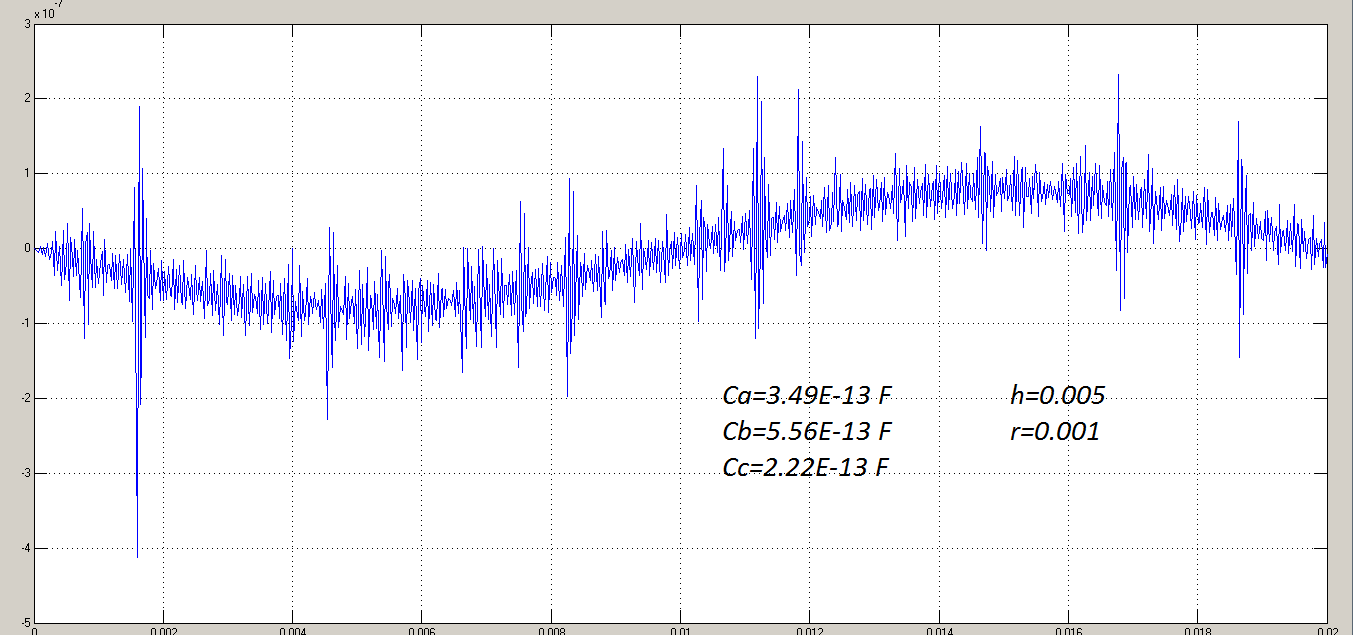
\includegraphics[width=\textwidth]{WaveformsforTransient2}
    \caption{Waveforms for Transient}
    \label{fig:Waveforms for Transient}
\end{figure}

The effect of transients can be seen in the waveform as compared to steady state waveforms.

The frequency of PD waveforms are higher

Intermitted increase in the amplitude of waveform due to transients. 

\pagebreak
\begin{center}
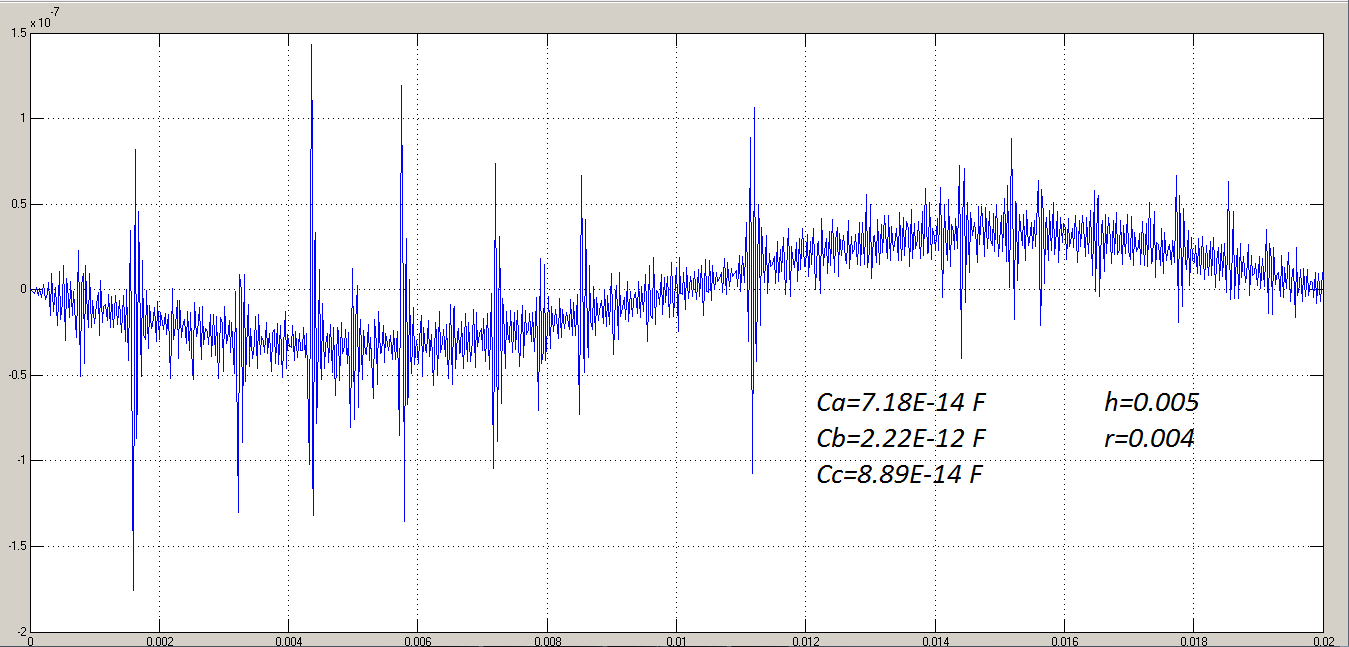
\includegraphics[width=\textwidth]{TWave1}
\vfill
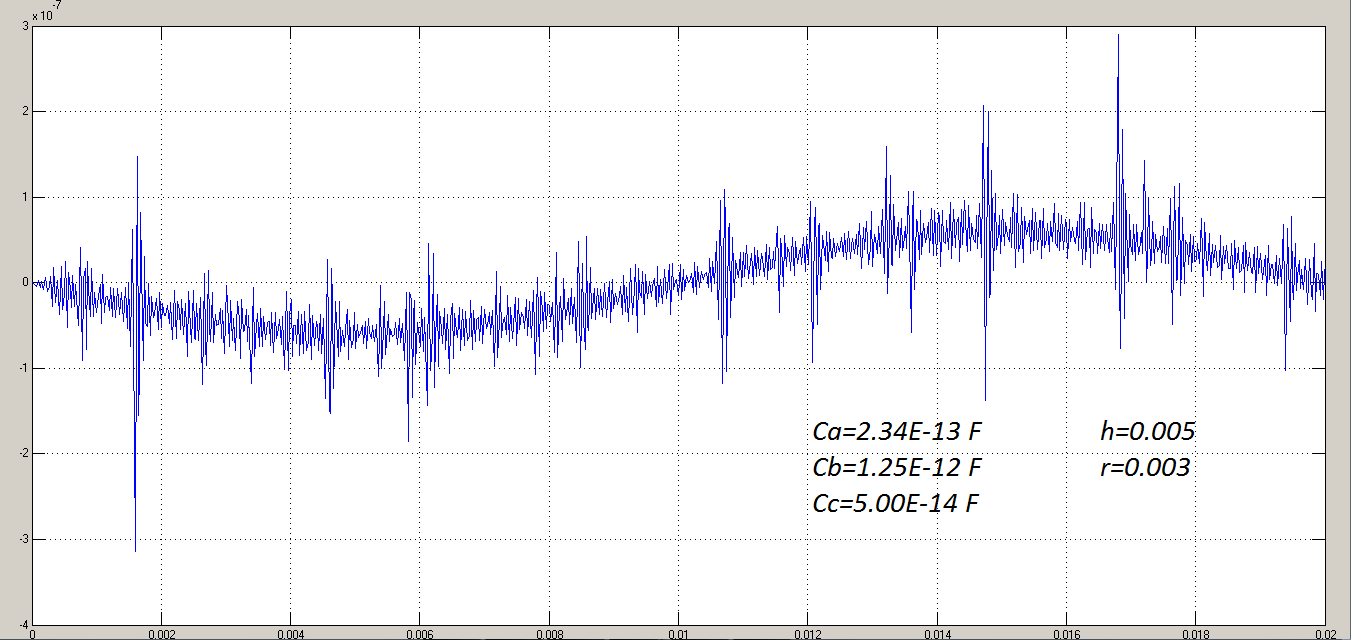
\includegraphics[width=\textwidth]{TWave2}
\vfill
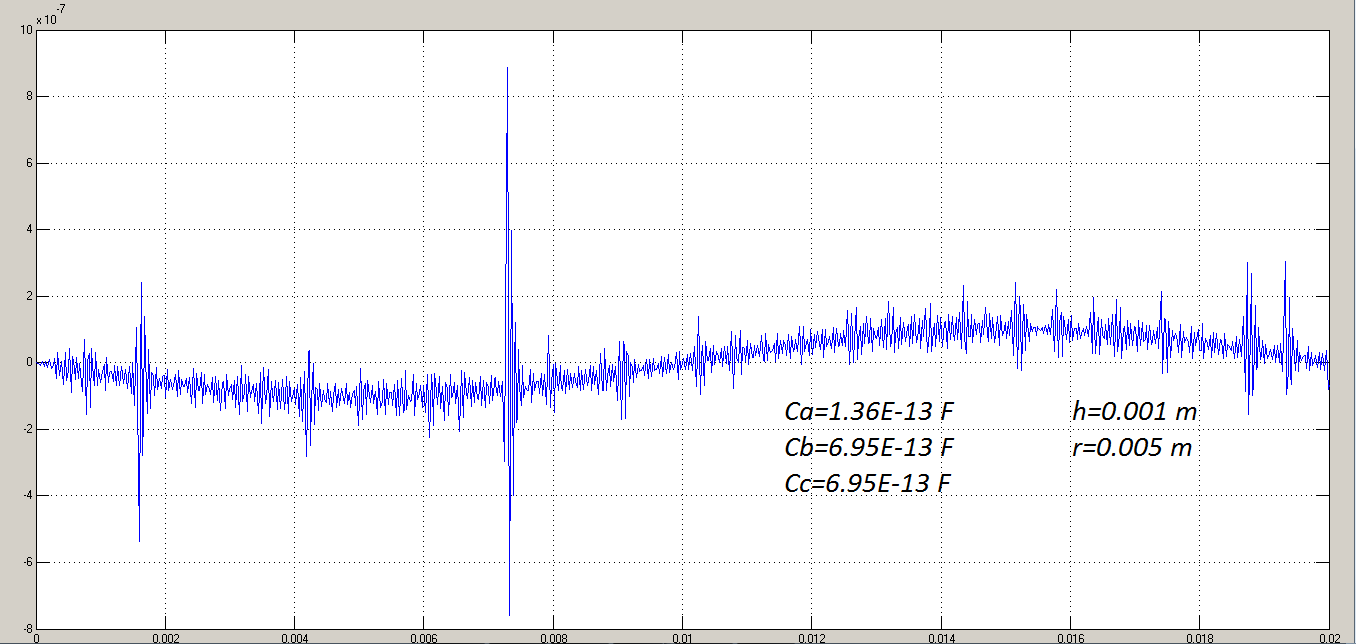
\includegraphics[width=\textwidth]{TWave3}
\end{center}


\pagebreak
\begin{center}
As the dimensions of void increases, the magnitude of PD Pulses is more.
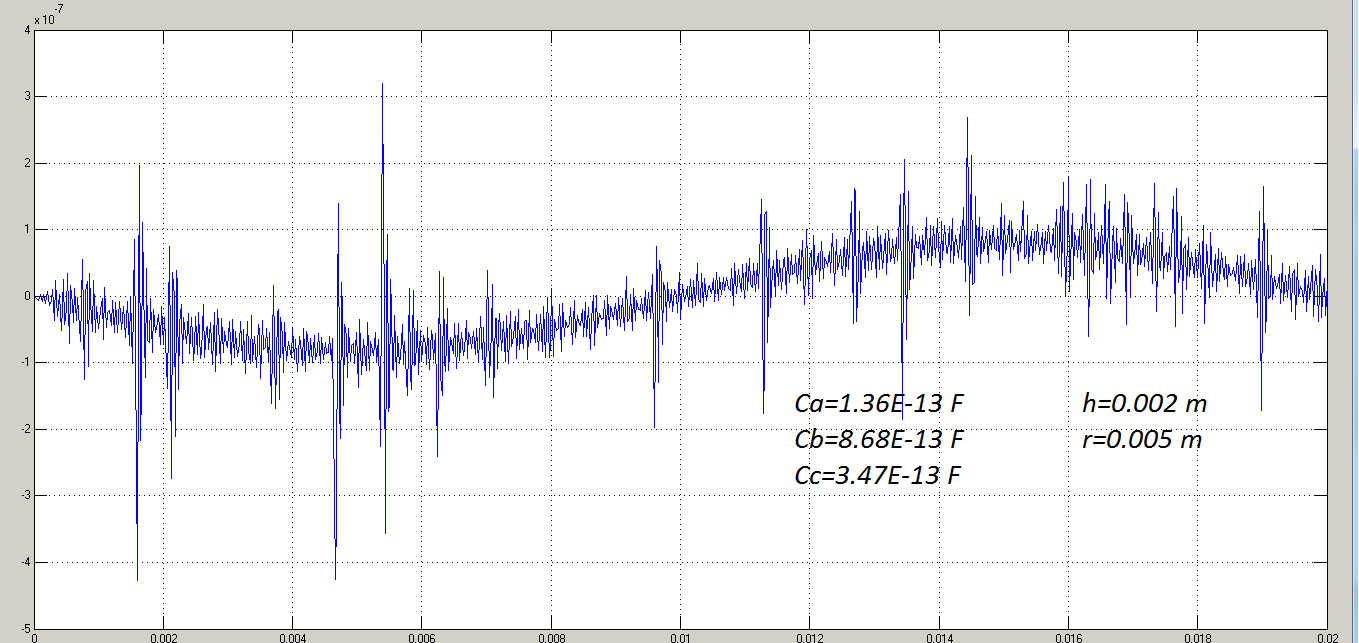
\includegraphics[width=\textwidth]{TWave4}
\vfill
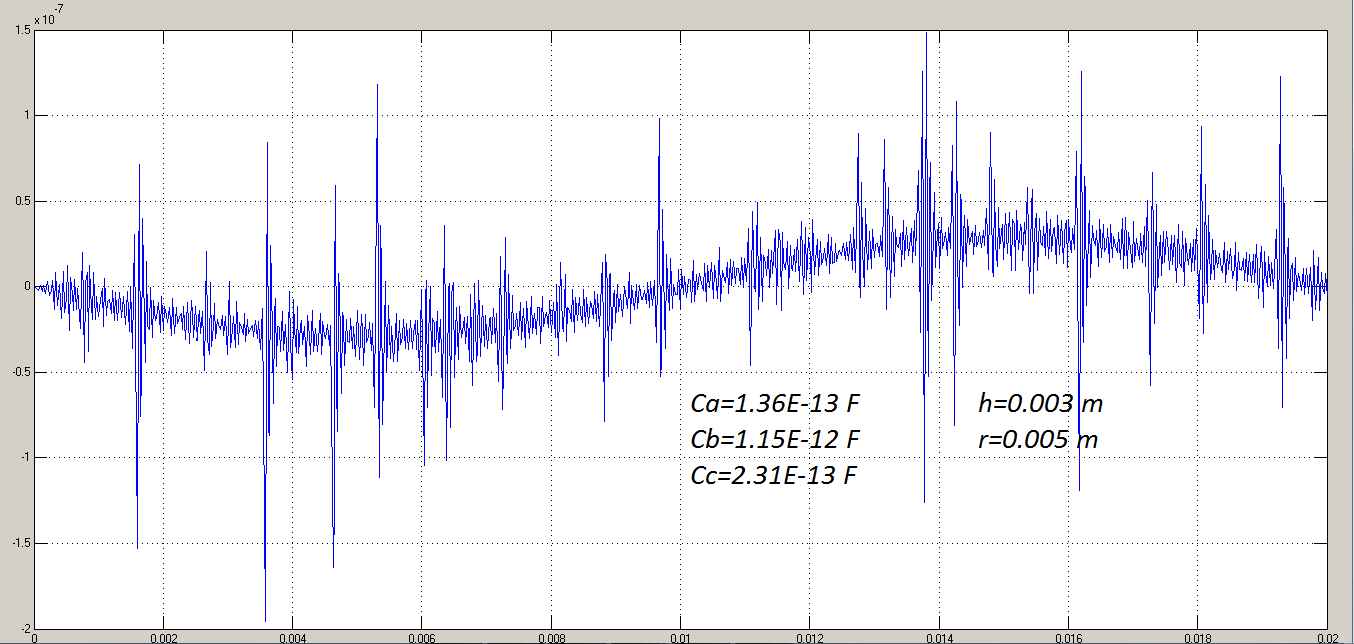
\includegraphics[width=\textwidth]{TWave5}
\vfill
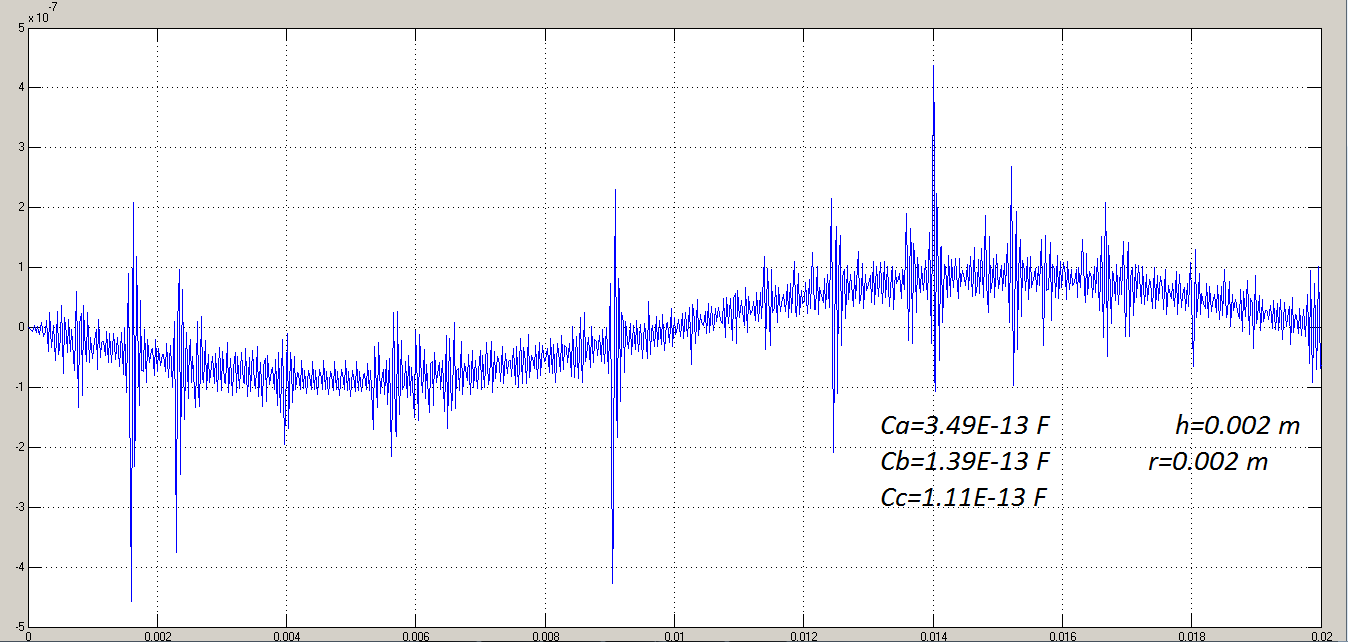
\includegraphics[width=\textwidth]{TWave6}
\end{center}

\pagebreak
\begin{center}
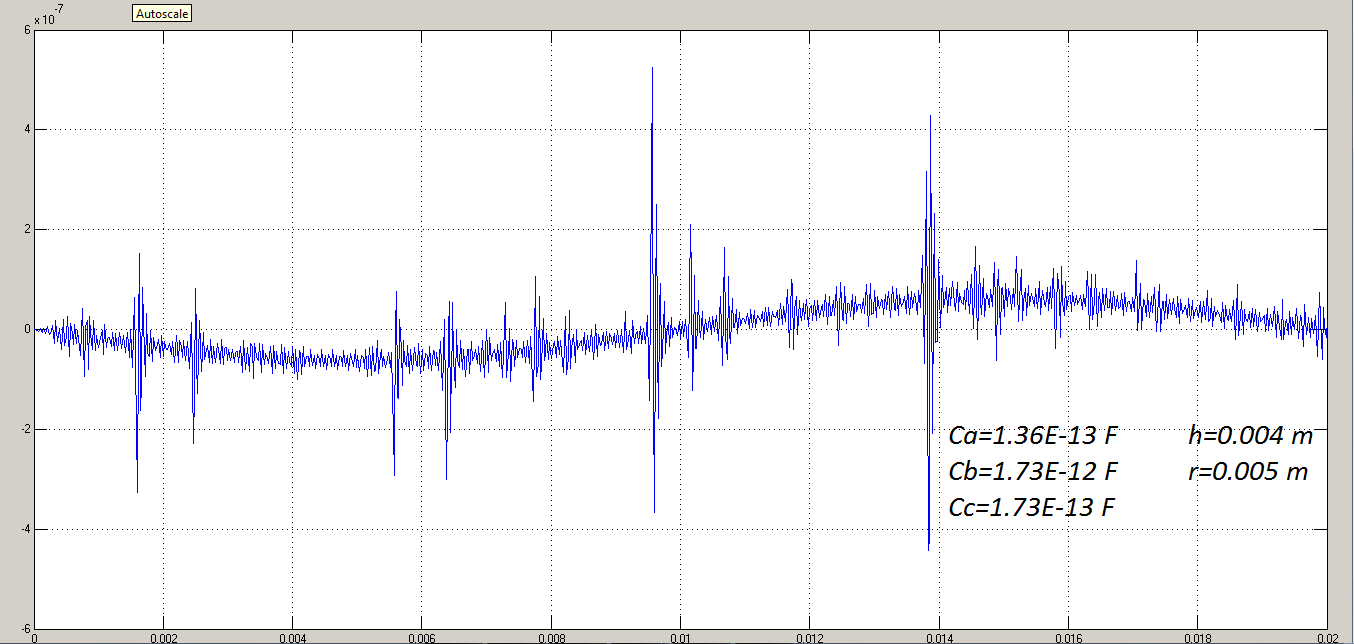
\includegraphics[width=\textwidth]{TWave7}
\vfill
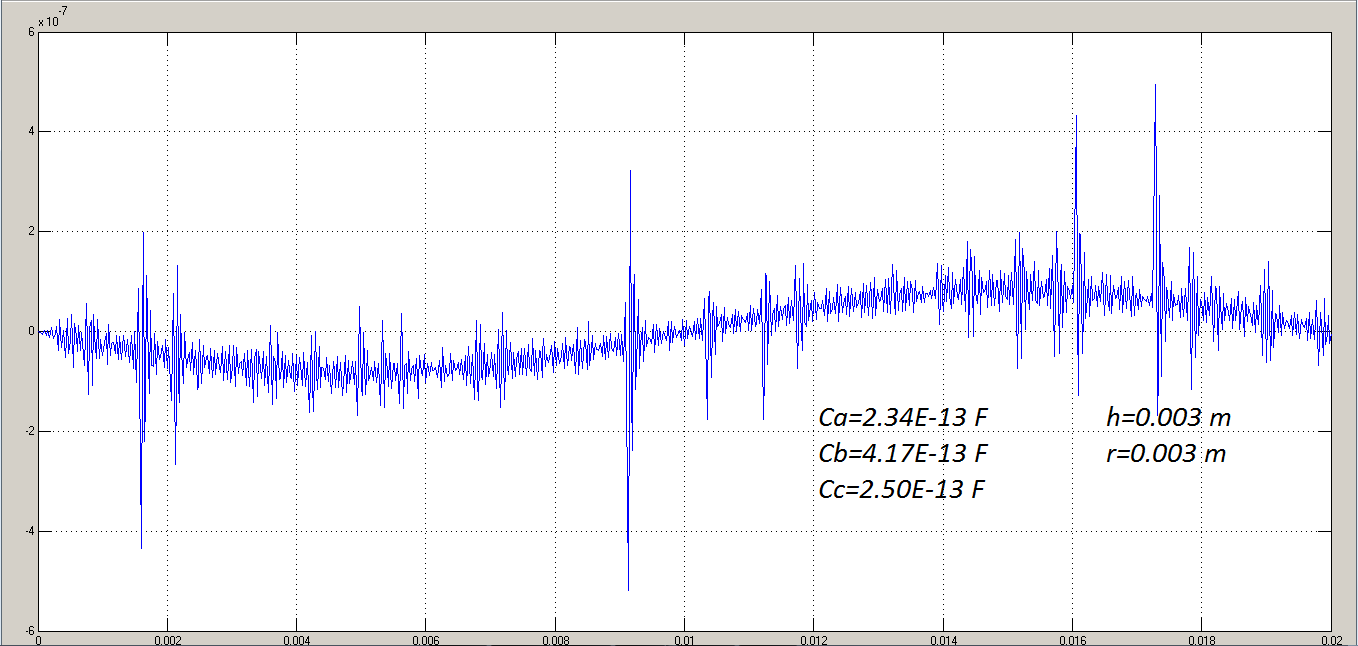
\includegraphics[width=\textwidth]{TWave8}
\vfill
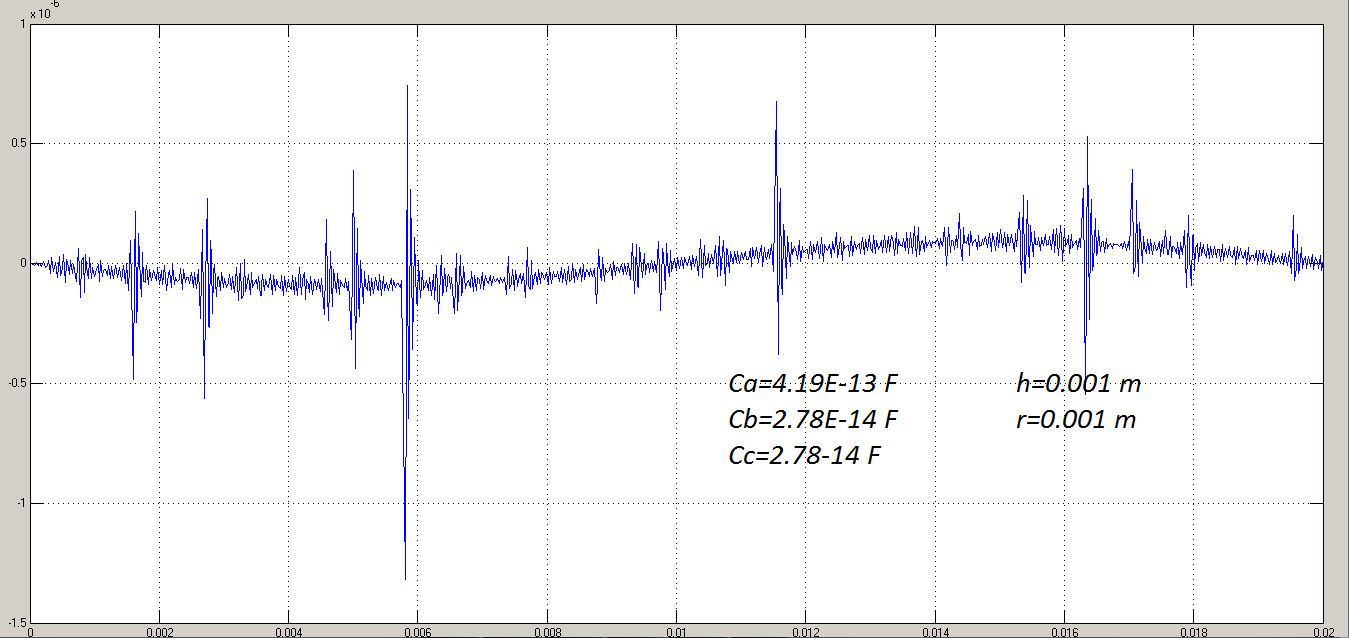
\includegraphics[width=\textwidth]{TWave9}
\vfill
A number of PD waveforms are more as the dimensions of the void are increased. 
\end{center}

\pagebreak
\begin{center}
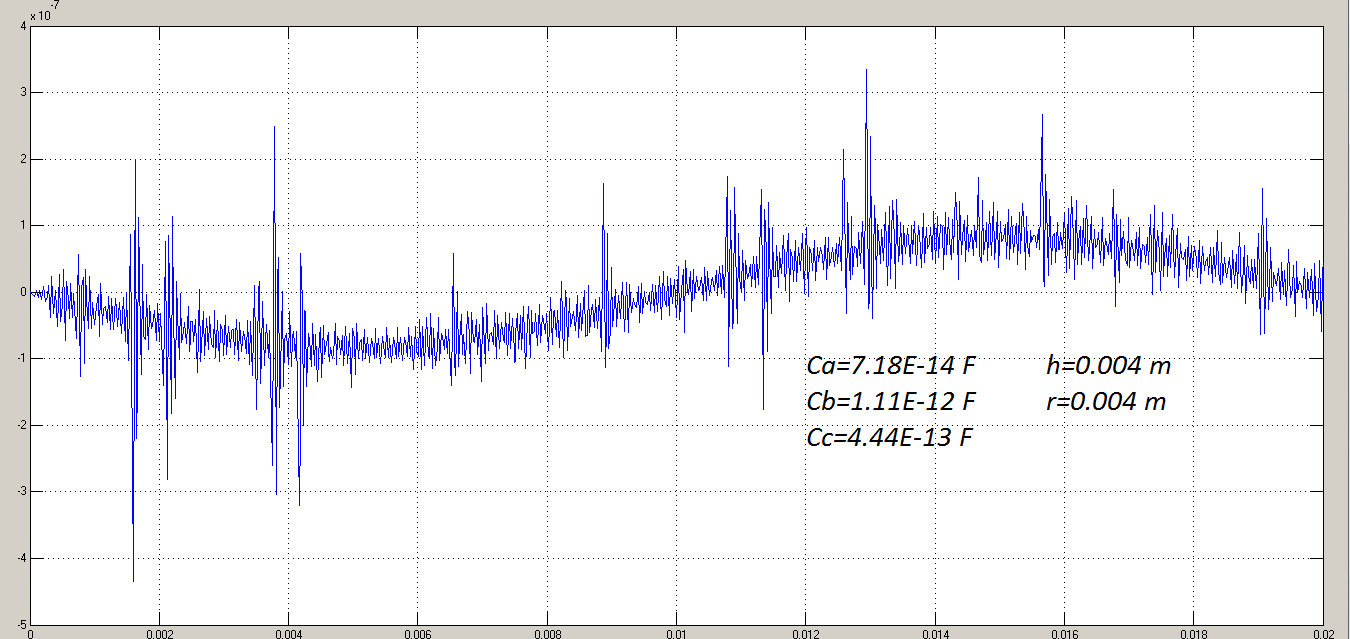
\includegraphics[width=\textwidth]{TWaveA}
\vfill
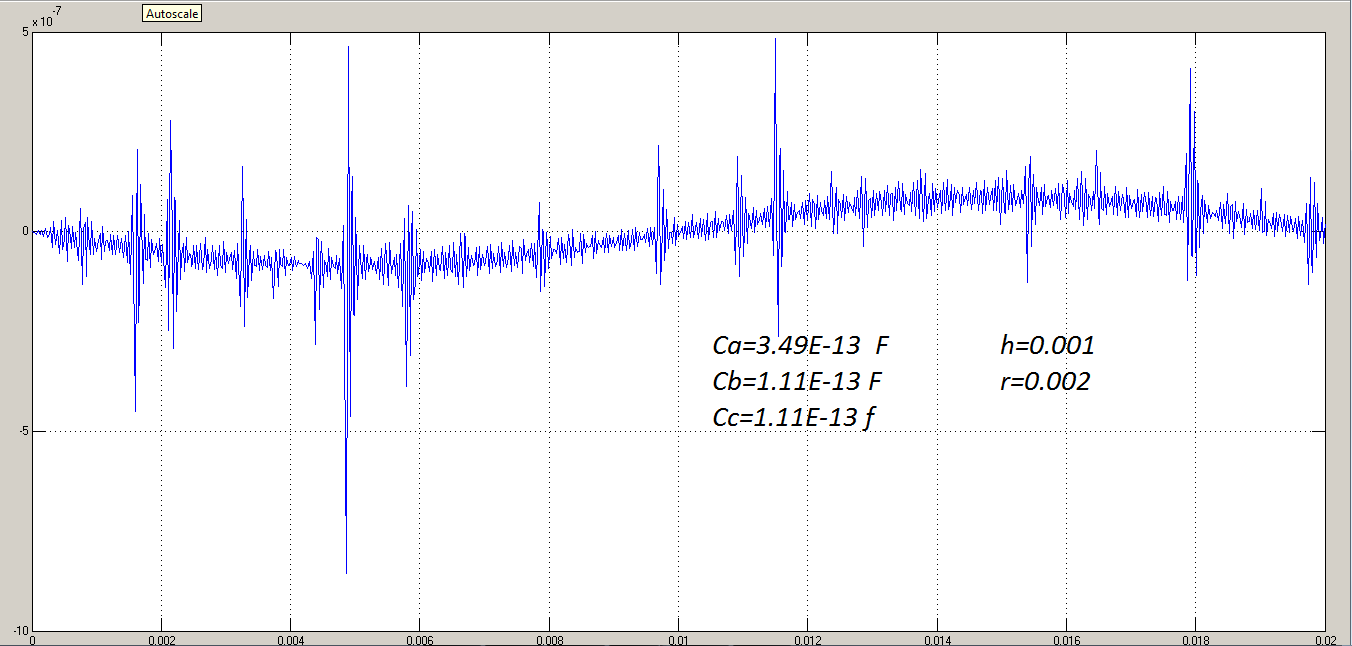
\includegraphics[width=\textwidth]{TWaveB}
\vfill
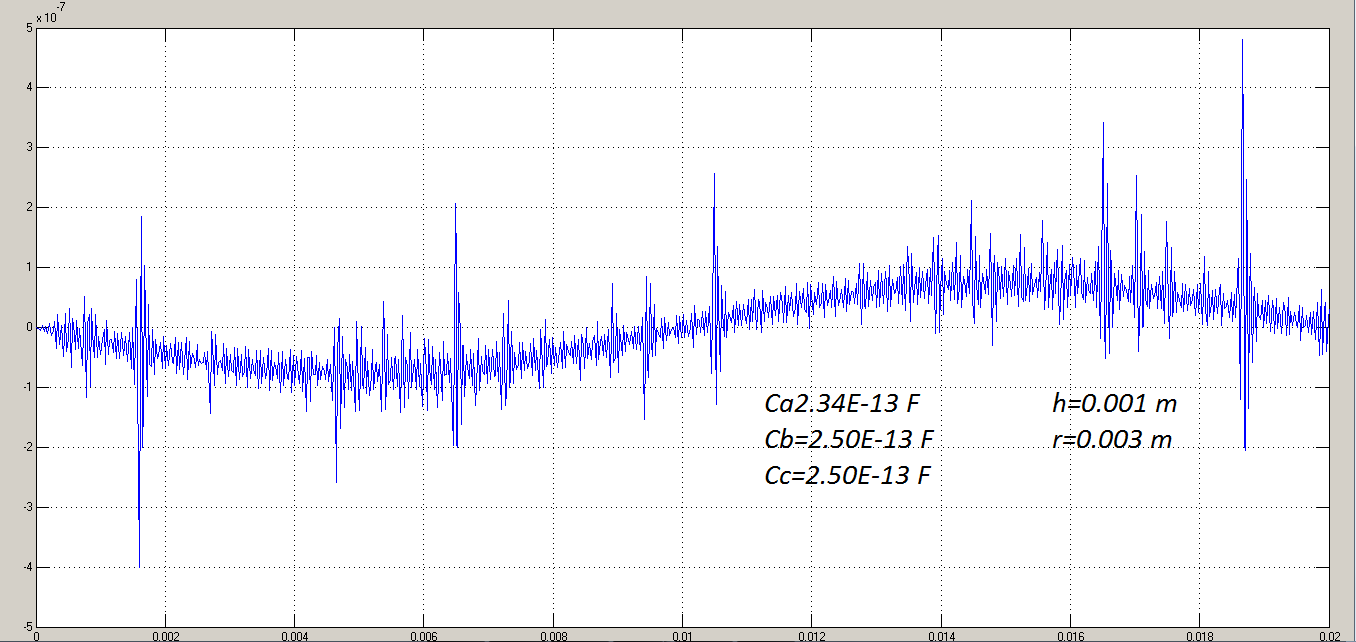
\includegraphics[width=\textwidth]{TWaveC}
\end{center}

\pagebreak
\begin{center}
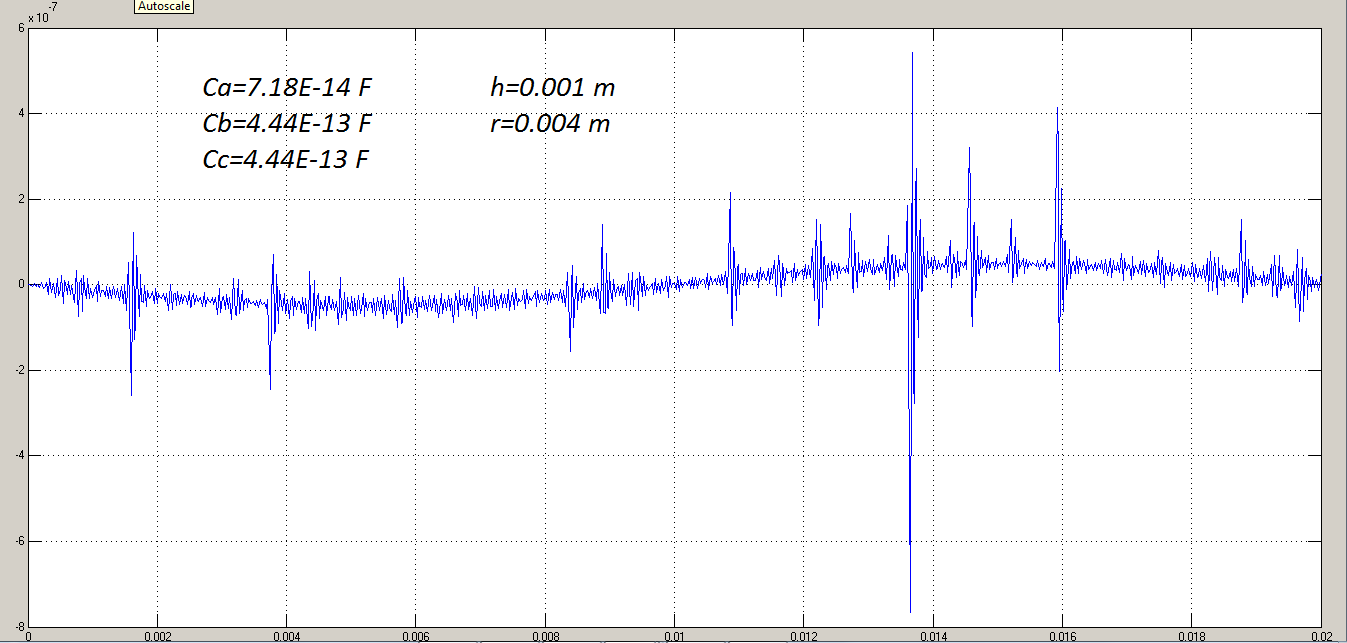
\includegraphics[width=\textwidth]{TWaveD}
\vfill
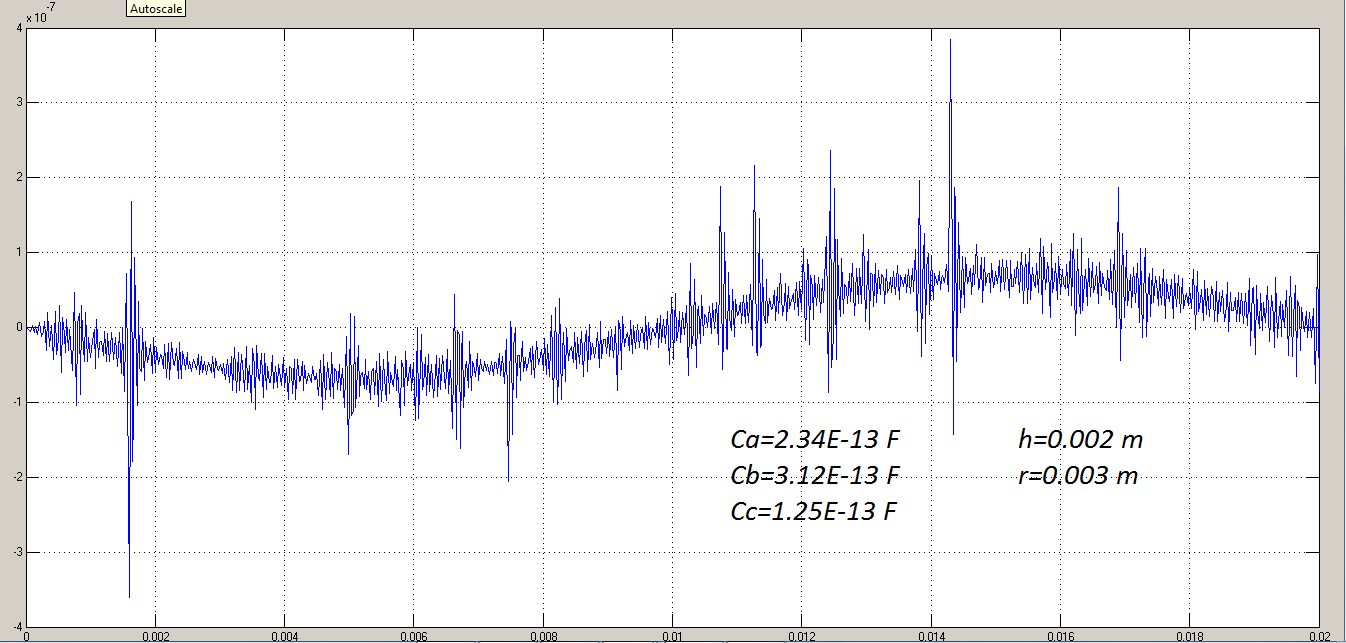
\includegraphics[width=\textwidth]{TWaveE}
\vfill
\includegraphics[width=\textwidth]{TWaveF}
\vfill
Distribution of PD Pulses is nonuniform for different void sizes.
\end{center}

\pagebreak
\begin{center}
\includegraphics[width=\textwidth]{TWaveG}
\vfill
\includegraphics[width=\textwidth]{TWaveH}
\vfill
\includegraphics[width=\textwidth]{TWaveI}
\end{center}

\pagebreak
\begin{center}
\includegraphics[width=\textwidth]{TWaveJ}
\vfill
\includegraphics[width=\textwidth]{TWaveK}
\vfill
\includegraphics[width=\textwidth]{TWaveL}
\end{center}

\pagebreak
\begin{center}
\includegraphics[width=\textwidth]{TWaveM}
\vfill
\includegraphics[width=\textwidth]{TWaveN}
\vfill
\includegraphics[width=\textwidth]{TWaveO}
\vfill
For particular dimensions of void, a linear variation observed in PD Pulses.
\end{center}

\pagebreak
\begin{center}
\includegraphics[width=\textwidth]{TWaveP}
\vfill
\includegraphics[width=\textwidth]{TWaveQ}
\vfill
\includegraphics[width=\textwidth]{TWaveR}
\end{center}

\pagebreak
\begin{center}
\includegraphics[width=\textwidth]{TWaveS}\\
\vspace*{1in}
\includegraphics[width=\textwidth]{TWaveT}
\end{center}

\pagebreak
\section{Analytical Analysis}
Based on the developed system discussed in chapter 3, a comprehensive analytical analysis is done for the following models considering the given mathematical equations and solving for steady state and short circuit and transient conditions\setlength{\parskip}{1em}.

\begin{enumerate}
\item Apparent charge 
\item Dimensions of voids
\item Accuracy of current transformers
\end{enumerate}

The dimensions of voids considered of various sizes from 0.001 m to 0.004 m as the volume of void increases, the capacitance increase, and the apparent charge increases. The effect on the phenomenon of partial discharge will lead to the formation of arcs . The deterioration of insulation takes place and can be evident from the partial discharge pulses.

\begin{enumerate}
\item Representation of voids in Capacitance 
\item Partial discharge pulse 
\end{enumerate}

The waveforms discussed in this chapter for during steady state conditions and transient conditions shows the intensity of partial discharge pulses. The intensity of pulse varies with the increase in capacitance of voids. The overall capacitance of void increases, the electrical stress in void increases due to this discharge increases to the extent of breakdown of the void \cite{bengtsson1997procedure}.

The waveforms due to transients show dense concentration of waves shows the partial discharge intensity. This intensity varies with the increase in capacitance, \textit{i.e.}, dimension of voids. These pulses were analyzed for void size varying from 0.001 m to 0.005 m. The amplitude, peak of the pulses, density of discharges can be evident to distinguish of pulse waveform for same voids in steady state operation of current transformers. 

The Capacitance values $C_a$, $C_b$, $C_c$ are calculated, and same values are used in Simulink Model for waveform pulses.

\begin{table}[h!]
\caption{Calculated Values of Capacitance 1}
\label{table:Calculated Values of Capacitance 1}
\centering
\begin{tabular}{|c|c|c|c|c|c|}
\hline 
Height of void 	&Radius of void &Sample dimension 				&$C_a$			&$C_b$			&$C_c$         \\ 
	(m)			&	(m) 		&								&(Farad) 		&(Farad) 		&(Farad)       \\ \hline \hline
0.005			&0.001			&.020$\times$.030$\times$.05 	&4.19$e^{-13}$	&1.39$e^{-13}$	&5.56$e^{-15}$ \\ \hline
0.005			&0.002			&.020$\times$.030$\times$.05 	&3.49$e^{-13}$	&5.56$e^{-13}$	&2.22$e^{-14}$ \\ \hline
0.005			&0.003			&.020$\times$.030$\times$.05 	&2.34$e^{-13}$	&1.25$e^{-12}$	&5.00$e^{-14}$ \\ \hline
0.005			&0.004			&.020$\times$.030$\times$.05 	&7.18$e^{-14}$	&2.22$e^{-12}$	&8.89$e^{-14}$ \\ \hline
0.005			&0.005			&.020$\times$.030$\times$.05 	&1.36$e^{-13}$	&3.47$e^{-12}$	&1.39$e^{-13}$ \\ \hline
\end{tabular} 
\end{table}

\begin{table}[h!]
\caption{Calculated Values of Capacitance 2}
\label{table:Calculated Values of Capacitance 2}
\centering
\begin{tabular}{|c|c|c|c|c|c|c|}
\hline 
Void & Void & Dimensions & \multicolumn{3}{c|}{Capacitance}  \\ 
\hline 
Geometry & Height & Radius &  All Insulation & Series with Void & Void \\  
• & m & m &  $C_a F$ & $C_b F$ & $C_c F$ \\ \hline \hline
\multirow{4}{*}{Ellipse}& 0.002	& 0.005	& 1.37$e^{-13}$	& 8.69$e^{-13}$	& 3.48$e^{-13}$ \\  \cline{2-6}
 		& 0.003	& 0.004	& 7.19$e^{-14}$	& 7.41$e^{-13}$	& 1.48$e^{-13}$ \\ \cline{2-6}
 		& 0.003	& 0.005	& 1.37$e^{-13}$	& 1.16$e^{-12}$	& 2.32$e^{-13}$ \\ \cline{2-6}
 		& 0.004	& 0.005	& 1.37$e^{-13}$	& 1.74$e^{-12}$	& 1.74$e^{-13}$ \\ \hline
\end{tabular} 
\end{table}

\begin{table}[h!]
\caption{Calculated Values of Capacitance 3}
\label{table:Calculated Values of Capacitance 3}
\centering
\begin{tabular}{|c|c|c|c|c|c|c|}
\hline 
Void & \multicolumn{3}{c|}{Void Dimensions} & \multicolumn{3}{c|}{Capacitance}  \\ 
\hline 
Geometry & Height & Radius & Area &  All Insulation & Series with Void & Void \\ 
• & m & m & m\textsuperscript{2} & $C_a F$ & $C_b F$ & $C_c F$ \\ \hline \hline 
			&0.005	&0.001	&0.0000032	&4.19$e^{-13}$	&1.39$e^{-13}$	&2.39$e^{-12}$ \\ \cline{2-7}
Irregular	&0.005	&0.002	&0.0000039	&3.50$e^{-13}$	&5.56$e^{-13}$	&9.62$e^{-12}$ \\ \cline{2-7}
 Shape		&0.005	&0.003	&0.0000045	&2.34$e^{-13}$	&1.25$e^{-12}$	&2.17$e^{-11}$ \\ \cline{2-7}
 			&0.005	&0.004	&0.0000055	&7.19$e^{-14}$	&2.22$e^{-12}$	&3.86$e^{-11}$ \\ \cline{2-7}
 			&0.005	&0.005	&0.0000032	&1.37$e^{-13}$	&3.48$e^{-12}$	&6.03$e^{-11}$ \\ \hline
\end{tabular} 
\end{table}

The capacitance values $C_a$, $C_b$, $C_c$ changes with void sizes. Capacitances values are calculated. Pulse waveforms for these waveforms show partial discharge phenomenon.

Relationship of Apparent charge to the size of the void is tabulated in the Table \ref{table:Apparent Charge with Different Void Sizes}. It shows the linear relationship.

\begin{table}[h!]
\caption{Apparent Charge with Different Void Sizes}
\label{table:Apparent Charge with Different Void Sizes}
\centering
\begin{tabular}{|c|c|c|c|c|}
\hline 
\multicolumn{3}{|c|}{Void Dimensions} &	Volume of Void	& Apparent Charge \\ \cline{1-3}
Height & Radius & Depth &  &  \\
m	&m	&m	& 	& 	\\ \hline \hline
0.005	&0.001	&0.001	&5$e^{-9}$&	2.00$e^{-14}$\\ \hline
0.005	&0.002	&0.001	&1$e^{-8}$&	3.88$e^{-14}$\\ \hline
0.005	&0.003	&0.001	&1.5$e^{-8}$&	5.67$e^{-14}$\\ \hline
0.005	&0.004	&0.001	&2$e^{-8}$&	7.98$e^{-14}$\\ \hline
0.005	&0.005	&0.001	&2.5$e^{-8}$&	9.83$e^{-14}$\\ \hline \hline
 	 	 	 	 
0.001	&0.001	&0.001	&1$e^{-9}$&	4.01$e^{-15}$\\ \hline
0.002	&0.002	&0.001	&4$e^{-9}$&	1.58$e^{-14}$\\ \hline
0.003	&0.003	&0.001	&9$e^{-9}$&	3.62$e^{-14}$\\ \hline
0.004	&0.004	&0.001	&1.6$e^{-8}$&	6.36$e^{-14}$\\ \hline
\end{tabular} 
\end{table}

Calculated values of Capacitance and waveforms from Simulink model shows the resemblance in the characteristics. 
\clearpage

\section[Comparison between Computational and Analytical Analysis]{Comparison between Computational and\\Analytical Analysis}
In all the models considered for the study during steady state and transients, the accuracy of current transformers changes considerably as the dielectric strength of insulating material changes which reflects in the performance and applications.

Enclosed readings of the accuracy of current transformers for various class. The accuracy performance of current transformers in steady state abruptly varies with the occurrence of transients.

\begin{table}[h!]
\caption{Accuracy Results of Different CT class}
\label{table:Accuracy Results of Different CT class}
\centering
\begin{tabular}{|c|c|c|c|c|}
\hline 
Sr. & CT Ratio Class	& Primary Current	& Steady state Ratio	& Transients Ratio \\
No. &					& \% 				& Error \% 				&  Error \% 		\\ \hline \hline
1	&0.5 S	& 		& 			& 			\\ \hline 
 	&3000/1 & 120	&	0.342	& 2.345 	\\ \hline 
 	&		& 100	&	0.331	& 2.456	\\ \hline 
 	&		& 20	& 0.129	& 1.341	\\ \hline 
 	&		& 5		& 0.012	&1.456	\\ \hline 
 	&		&120	&0.256	&2.023	\\ \hline 
 	&		&100	&0.237	&2.402	\\ \hline 
 	&		&20		&0.148	&1.890	\\ \hline 
 	&		&5		&0.126	&1.562	\\ \hline \hline
2	&PS		& 		& 			&			\\ \hline  
 	&2400/1	&100	&-0.034	&5.670	\\ \hline \hline
3	&5P		& 		& 			& 			\\ \hline 
 	&600/5	&100	&0.007	&3.15		\\ \hline \hline
4	&0.2 S	& 		& 			& 			\\ \hline 
 	&200/1	& 120	&0.116	&1.568	\\ \hline 
 	& 		& 100	&0.112	&1.558	\\ \hline 
 	& 		& 20	&0.076	&2.321	\\ \hline
 	&		& 5		&0.053	&2.291	\\ \hline
 	& 		& 120	&0.158	&1.628	\\ \hline
 	& 		& 100	&0.157	&1.601	\\ \hline
 	& 		& 20	&0.153	&1.289	\\ \hline
 	& 		& 5		&0.144	&1.243	\\ \hline
\end{tabular} 
\end{table}

The waveforms generated for various sizes of voids in the Simulink model in steady state and transients also shows the variations in partial discharge pulses resulting in the deterioration of the performance of current transformers. The amplitude, pulse, spike, density of partial discharge, frequency is shown in all waveforms are compared for the same void sizes in steady state and transient conditions. The distortion in the waveform is significant.

The results of performance distortion of oil filled current transformers 145 kV up to 3000 A by the computational method and analytical method shows same relevance in steady state and transient conditions due to the voids in insulating material or occurrence of partial discharge.  
\clearpage

\section{Justification for the difference}
The difference in the results obtained by the computational analysis and the analytical analysis discussed above is because one represents the performance regarding the numerical values and the other represents the performance in the wave form pulses. The computational analysis gives the distorted waveforms for the different values using the MATLAB/Simulink software is used for the simulation\setlength{\parskip}{0em}.